\documentclass{beamer}

% Beamer style
%\usetheme[secheader]{Madrid}
\usetheme{CambridgeUS}
\usecolortheme[rgb={0.65,0.15,0.25}]{structure}
%\usefonttheme[onlymath]{serif}
\beamertemplatenavigationsymbolsempty
%\AtBeginSubsection

% Packages
%\usepackage[french]{babel}
\usepackage[latin1]{inputenc}
\usepackage{color}
%\usepackage{dsfont, stmaryrd}
\usepackage{amsmath, amsfonts, amssymb}
\usepackage{epsfig}
\usepackage{url}
\usepackage{/home/robin/LATEX/astats}
%\usepackage[all]{xy}
\usepackage{graphicx}

% Commands
\definecolor{darkred}{rgb}{0.65,0.15,0.25}
\newcommand{\emphase}[1]{\textcolor{darkred}{#1}}
%\newcommand{\emphase}[1]{{#1}}
\newcommand{\paragraph}[1]{\textcolor{darkred}{#1}}
\newcommand{\refer}[1]{[{\footnotesize{\textcolor{blue}{{\cite{#1}}}}}]}
\newcommand{\Refer}[1]{[{\footnotesize{\textcolor{blue}{{\sl #1}}}}]}
\newcommand{\newblock}{}

% Symbols
\newcommand{\Abf}{{\bf A}}
\newcommand{\Beta}{\text{B}}
\newcommand{\Bcal}{\mathcal{B}}
\newcommand{\BIC}{\text{BIC}}
\newcommand{\Ccal}{\mathcal{C}}
\newcommand{\dd}{\text{~d}}
\newcommand{\dbf}{{\bf d}}
\newcommand{\Dcal}{\mathcal{D}}
\newcommand{\Esp}{\mathbb{E}}
\newcommand{\Ebf}{{\bf E}}
\newcommand{\Ecal}{\mathcal{E}}
\newcommand{\Gcal}{\mathcal{G}}
\newcommand{\Gam}{\mathcal{G}\text{am}}
\newcommand{\Ibb}{\mathbb{I}}
\newcommand{\Ibf}{{\bf I}}
\newcommand{\ICL}{\text{ICL}}
\newcommand{\Cov}{\mathbb{C}\text{ov}}
\newcommand{\Corr}{\mathbb{C}\text{orr}}
\newcommand{\Var}{\mathbb{V}}
\newcommand{\Vsf}{\mathsf{V}}
\newcommand{\pen}{\text{pen}}
\newcommand{\Fcal}{\mathcal{F}}
\newcommand{\Hbf}{{\bf H}}
\newcommand{\Hcal}{\mathcal{H}}
\newcommand{\Jcal}{\mathcal{J}}
\newcommand{\Kbf}{{\bf K}}
\newcommand{\Lcal}{\mathcal{L}}
\newcommand{\Mcal}{\mathcal{M}}
\newcommand{\mbf}{{\bf m}}
\newcommand{\mum}{\mu(\mbf)}
\newcommand{\Ncal}{\mathcal{N}}
\newcommand{\Nbf}{{\bf N}}
\newcommand{\Nm}{N(\mbf)}
\newcommand{\Ocal}{\mathcal{O}}
\newcommand{\Obf}{{\bf 0}}
\newcommand{\Omegas}{\underset{s}{\Omega}}
\newcommand{\Pbf}{{\bf P}}
\newcommand{\Pcal}{\mathcal{P}}
\newcommand{\Qcal}{\mathcal{Q}}
\newcommand{\Rbb}{\mathbb{R}}
\newcommand{\Rcal}{\mathcal{R}}
\newcommand{\sbf}{{\bf s}}
\newcommand{\Sbf}{{\bf S}}
\newcommand{\Scal}{\mathcal{S}}
\newcommand{\Ucal}{\mathcal{U}}
\newcommand{\Vcal}{\mathcal{V}}
\newcommand{\Tbf}{{\bf T}}
\newcommand{\ubf}{{\bf u}}
\newcommand{\Ubf}{{\bf U}}
\newcommand{\Wbf}{{\bf W}}
\newcommand{\xbf}{{\bf x}}
\newcommand{\Xbf}{{\bf X}}
\newcommand{\ybf}{{\bf y}}
\newcommand{\Ybf}{{\bf Y}}
\newcommand{\zbf}{{\bf z}}
\newcommand{\Zbf}{{\bf Z}}
\newcommand{\betabf}{\text{\mathversion{bold}{$\beta$}}}
\newcommand{\pibf}{\text{\mathversion{bold}{$\pi$}}}
\newcommand{\phibf}{\text{\mathversion{bold}{$\phi$}}}
\newcommand{\Sigmabf}{\text{\mathversion{bold}{$\Sigma$}}}
\newcommand{\gammabf}{\text{\mathversion{bold}{$\gamma$}}}
\newcommand{\mubf}{\text{\mathversion{bold}{$\mu$}}}
\newcommand{\nubf}{\text{\mathversion{bold}{$\nu$}}}
\newcommand{\Thetabf}{\text{\mathversion{bold}{$\Theta$}}}
\newcommand{\thetabf}{\text{\mathversion{bold}{$\theta$}}}
\newcommand{\BP}{\text{BP}}
\newcommand{\EM}{\text{EM}}
\newcommand{\VEM}{\text{VEM}}
\newcommand{\VBEM}{\text{VBEM}}
\newcommand{\cst}{\text{cst}}
\newcommand{\obs}{\text{obs}}
\newcommand{\ra}{\emphase{\mathversion{bold}{$\rightarrow$}~}}
\newcommand{\QZ}{Q_{\Zbf}}
\newcommand{\Qt}{Q_{\thetabf}}
%\newcommand{\transp}{\text{{\tiny $\top$}}}
\newcommand{\transp}{\text{{\tiny \mathversion{bold}{$\top$}}}}

% Directory
\newcommand{\figmixt}{/home/robin/ENSEIGN/COURS/MELANGE}
\newcommand{\figbma}{/home/robin/RECHERCHE/RUPTURES/MELANGE/Exemples/Grippe}
\newcommand{\fignet}{/home/robin/RECHERCHE/RESEAUX/EXPOSES/FIGURES}
\newcommand{\figeco}{/home/robin/RECHERCHE/ECOLOGIE/EXPOSES/FIGURES}
%\newcommand{\figmotif}{/home/robin/RECHERCHE/RESEAUX/Motifs/FIGURES}


%--------------------------------------------------------------------
\title[Variational (Bayes) inference]{Some elements of
  variational (Bayes) inference for latent variable models}   

\author{S. Robin}

\institute[AgroParisTech / INRA]{AgroParisTech / INRA \\
  \bigskip
  \begin{tabular}{ccccc}
    
\epsfig{file=\fignet/LogoINRA-Couleur.ps,
      width=2.5cm} & 
    \hspace{.5cm} &
    
\epsfig{file=\fignet/logagroptechsolo.eps,
      width=3.75cm} & 
    \hspace{.5cm} &
    
\epsfig{file=\fignet/logo-ssb.eps,
      width=2.5cm} \\ 
  \end{tabular} \\
  \bigskip
  }

\date[S�minaire Rochebrune]{S�minaire Rochebrune, April 2012,
  Rochebrune}
%--------------------------------------------------------------------

%--------------------------------------------------------------------
%--------------------------------------------------------------------
\begin{document}
%--------------------------------------------------------------------
%--------------------------------------------------------------------

%--------------------------------------------------------------------
\frame{\titlepage}

%--------------------------------------------------------------------
\frame{ \frametitle{Outline}
  \tableofcontents}

%--------------------------------------------------------------------
%--------------------------------------------------------------------
\section{Introduction}
\frame{\frametitle{Introduction}}
%--------------------------------------------------------------------
\frame{\frametitle{Looking for conditional distributions}

  Many hierarchical / graphical models involve unobserved ('hidden')
  variables $\Zbf$ (or parameters $\thetabf$).

  \bigskip
  Many inference strategies aim at or require to determine their
  conditional distribution given the observations $\Xbf$.

  \pause\bigskip\bigskip
  \paragraph{Examples.}
  \begin{itemize}
  \item Frequentist maximum likelihood for latent variable models via E-M: \\
    \ra requires to compute $P(\Zbf | \Xbf; \thetabf)$. \\~
  \item Bayesian inference: \\
    \ra aims at computing $P(\thetabf|\Xbf)$ or even $P(\Zbf, \thetabf|\Xbf)$.
  \end{itemize}
  }

%--------------------------------------------------------------------
%--------------------------------------------------------------------
\section{Two incomplete data models}
\frame{\frametitle{Two incomplete data models}}

%--------------------------------------------------------------------
\subsection*{Hidden Markov Model (HMM)}
%--------------------------------------------------------------------
\frame{\frametitle{Hidden Markov Model (HMM)}

  \begin{tabular}{cc}
    \hspace{-.5cm}
    \begin{tabular}{p{.45\textwidth}}
      \paragraph{Data.} $\Xbf = (X_t)$ observed along 'time'. \\
      ~\\
      \paragraph{Idea.} The distribution $X_t$ depends on some hidden $Z_t$.
    \end{tabular}
    & 
    \hspace{-1cm}
    \begin{tabular}{p{.4\textwidth}}
      \epsfig{file =
        \figmixt/Exemples/TilingChip/ChIP-chip_chr4-LogRatioExtrait.eps,  
      width=6cm, height=4cm, clip=}  
    \end{tabular}
  \end{tabular}

  \pause
  \paragraph{Model.}
  \begin{itemize}
  \item $\Zbf = (Z_t)$ is an homogeneous Markov chain with transition
    $\pibf$;
  \item Observations $\Xbf = (X_t)$ are independent given $\Zbf$;
  \item The distribution of $X_t$ depends on $Z_t$: $(X_t |Z_t=k) \sim
    f_k = f(\cdot; \gamma_k)$;
%  \item Parameters: $\thetabf = (\pibf, \gammabf)$. Classification: $\Zbf$.
  \end{itemize}
  }

%--------------------------------------------------------------------
\frame{\frametitle{Frequentist maximum likelihood inference}

  \paragraph{Likelihood.} The (log-)likelihood
  $$
  \log P(\Xbf; \thetabf) = \log \sum_{\zbf} P(\Xbf, \zbf; \thetabf)
  $$
  can not be computed.

  \pause\bigskip\bigskip
  \paragraph{E-M trick.} But it can be decomposed as
  $$
  \log P(\Xbf; \thetabf) = \log P(\Xbf, \Zbf; \thetabf) - \log
  P(\Zbf | \Xbf; \thetabf), 
  $$
  \pause the conditional expectation of which gives
  \begin{eqnarray*}
    \Esp[\log P(\Xbf;\thetabf)|\Xbf] & = & \Esp[\log P(\Xbf, \Zbf;
    \thetabf)|\Xbf] - \Esp[\log P(\Zbf | \Xbf; \thetabf)|\Xbf] \\ 
    \pause
    \log P(\Xbf; \thetabf) & = & \Esp[\log P(\Xbf, \Zbf;
    \thetabf)|\Xbf] + \Hcal[P(\Zbf | \Xbf; \thetabf)]
  \end{eqnarray*}
  where $\Hcal$ stands for the entropy.
  }

%--------------------------------------------------------------------
\frame{\frametitle{E-M algorithm}

  Aims at maximizing the log-likelihood
  $$
  \log P(\Xbf; \thetabf)
  $$
  through the alternation of two steps \refer{DLR77}
  \begin{itemize}
  \item \pause \emphase{E-step:} calculate $P(\Zbf|\Xbf)$ \\
    \ra not explicit \\
    \ra but calculable via the forward-backward recursion \\
    ~
  \item \pause \emphase{M-step:} maximize $\Esp[\log P(\Xbf, \Zbf;
    \thetabf)|\Xbf]$ with respect to $\theta$ \\
    \ra generally similar to standard MLE.
  \end{itemize}
  }

%--------------------------------------------------------------------
\frame{\frametitle{Conditional distribution}

  \begin{tabular}{cc}
    \hspace{-.5cm}
    \begin{tabular}{p{.5\textwidth}}
      \onslide+<2->{\paragraph{Frequentist inference.}         
        \begin{itemize}
        \item The dependency graph is a tree;}
        \onslide+<3->{
        \item The moral graph is still a tree;}
        \onslide+<4->{
        \item $P(\Zbf|\Xbf)$ can be computed efficiently.
        \end{itemize}}
      \onslide+<5->{\bigskip
        \paragraph{Bayesian inference.}         
        \begin{itemize}
        \item The dependency graph is not a tree;}          
        \onslide+<6->{
        \item The moral graph is not a tree ($\Zbf$ and $\thetabf$
          are not conditionally independent);} 
        \onslide+<7->{
        \item $P(\Zbf, \thetabf|\Xbf)$ can not be computed efficiently.
        \end{itemize}}
    \end{tabular}
    & 
    \hspace{-.5cm}
    \begin{tabular}{p{.45\textwidth}}
      \paragraph{Graphical model representation.} \\ ~\\
      \begin{overprint}
        \onslide<2>
%        Dependency graph: \\~\\
        \epsfig{file = \fignet/FigHMM-GM-Freq-1.eps,
          width=.7\textwidth, clip=}   
        \onslide<3>
%        Moral graph: \\~\\
        \epsfig{file = \fignet/FigHMM-GM-Freq-2.eps,
          width=.7\textwidth, clip=}   
        \onslide<4>
%        Conditional dependency graph: \\~\\
        \epsfig{file = \fignet/FigHMM-GM-Freq-3.eps,
          width=.7\textwidth, clip=}   
        \onslide<5>
%        Dependency graph: \\~\\
        \epsfig{file = \fignet/FigHMM-GM-Bayes-1.eps,
          width=.7\textwidth, clip=}   
%        \onslide<6>
%        \epsfig{file = \fignet/FigHMM-GM-Bayes-2.eps,
%          width=.7\textwidth, clip=}   
        \onslide<6>
%        Moral graph: \\~\\
        \epsfig{file = \fignet/FigHMM-GM-Bayes-3.eps,
          width=.7\textwidth, clip=}   
        \onslide<7->
%        Conditional dependency graph: \\~\\
        \epsfig{file = \fignet/FigHMM-GM-Bayes-4.eps,
          width=.7\textwidth, clip=} \\
      \end{overprint}
      \onslide+<8>{\vspace{-1.5cm}
        \ra Variational methods can be used to approximate it.}
    \end{tabular}
  \end{tabular}
  }

%--------------------------------------------------------------------
\subsection*{Stochastic Block Model (SBM)}
%--------------------------------------------------------------------
\frame{\frametitle{Stochastic Block Model (SBM)}

  \begin{tabular}{cc}
    \hspace{-.5cm}
    \begin{tabular}{p{.5\textwidth}}
      \onslide+<1->{\paragraph{A mixture model for random graphs.}}
      \onslide+<2->{\begin{itemize}
        \item Consider $n$ nodes ($i = 1..n$); \\ ~ } 
        \onslide+<3->{
        \item $Z_i = $ unobserved label of node $i$:
          $$
          \{Z_i\} \text{ i.i.d. } \sim \Mcal(1; \pibf)
          $$
          $\pibf = (\pi_1, ... \pi_K)$; \\ ~ } 
        \onslide+<4->{
        \item Edge $X_{ij}$ depends on the labels:
          $\{X_{ij}\}$ independent given $\{Z_i\}$,
          $$
          (X_{ij}) \sim \Bcal(\gamma_{Z_i, Z_j})
          $$}
      \end{itemize}
    \end{tabular}
    & 
    \hspace{-.5cm}
    \begin{tabular}{p{.5\textwidth}}
      \vspace{1cm}
      \begin{overprint}
        \onslide<2>
        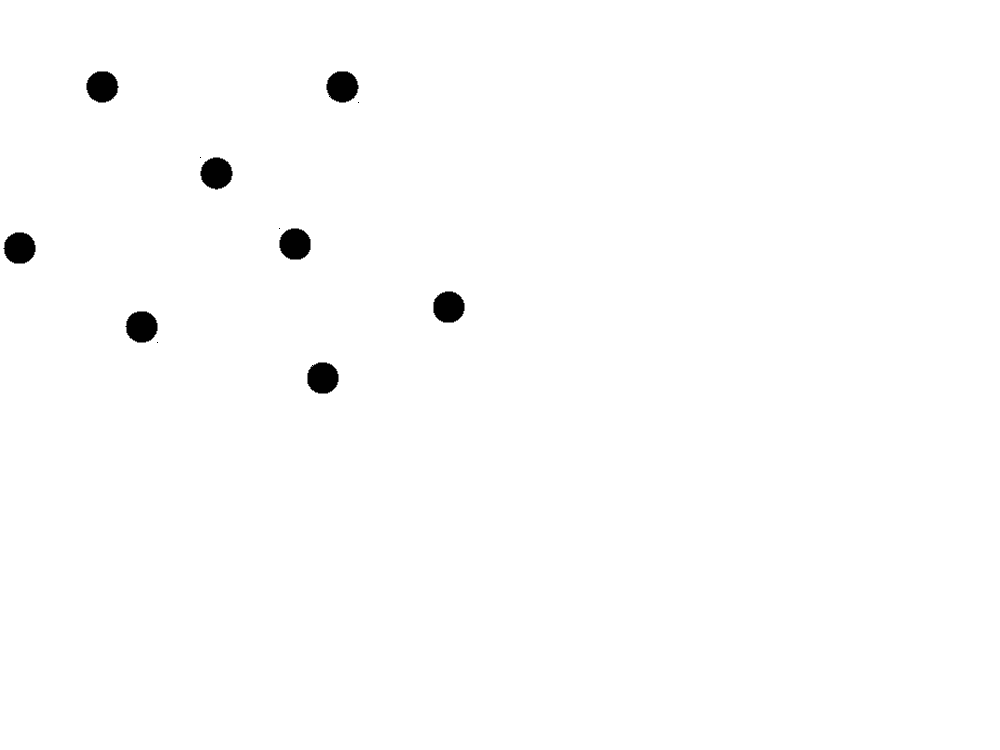
\epsfig{file = \fignet/FigSBM-Model-1.eps,
          width=.75\textwidth, clip=}    
        \onslide<3>
        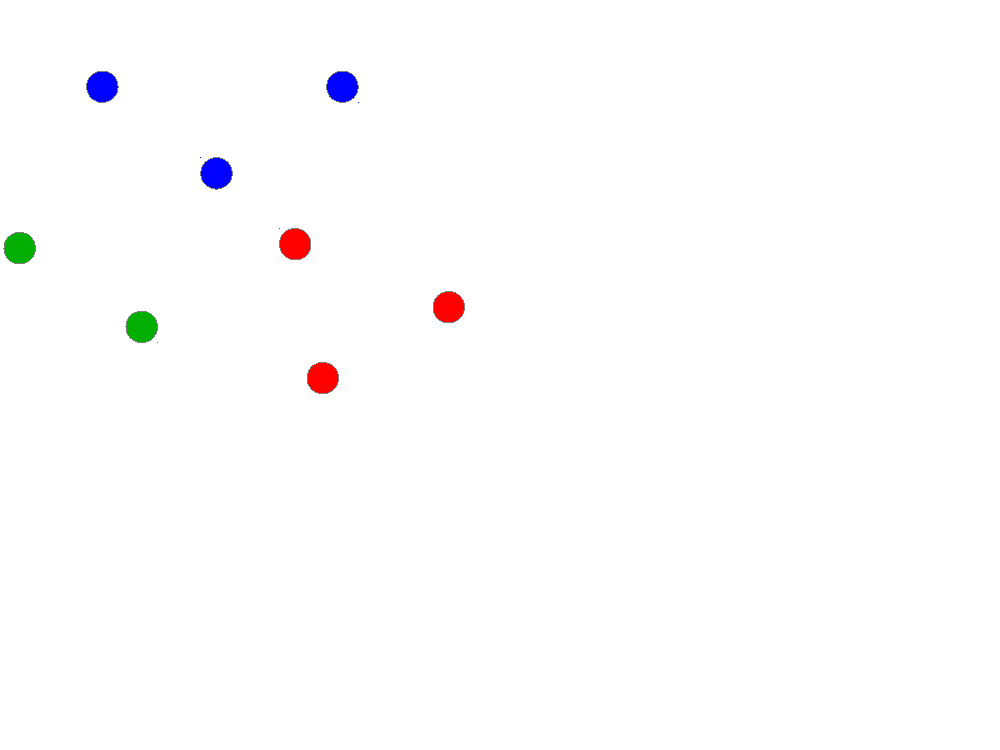
\epsfig{file = \fignet/FigSBM-Model-2.eps,
          width=.75\textwidth, clip=}    
        \onslide<4>
        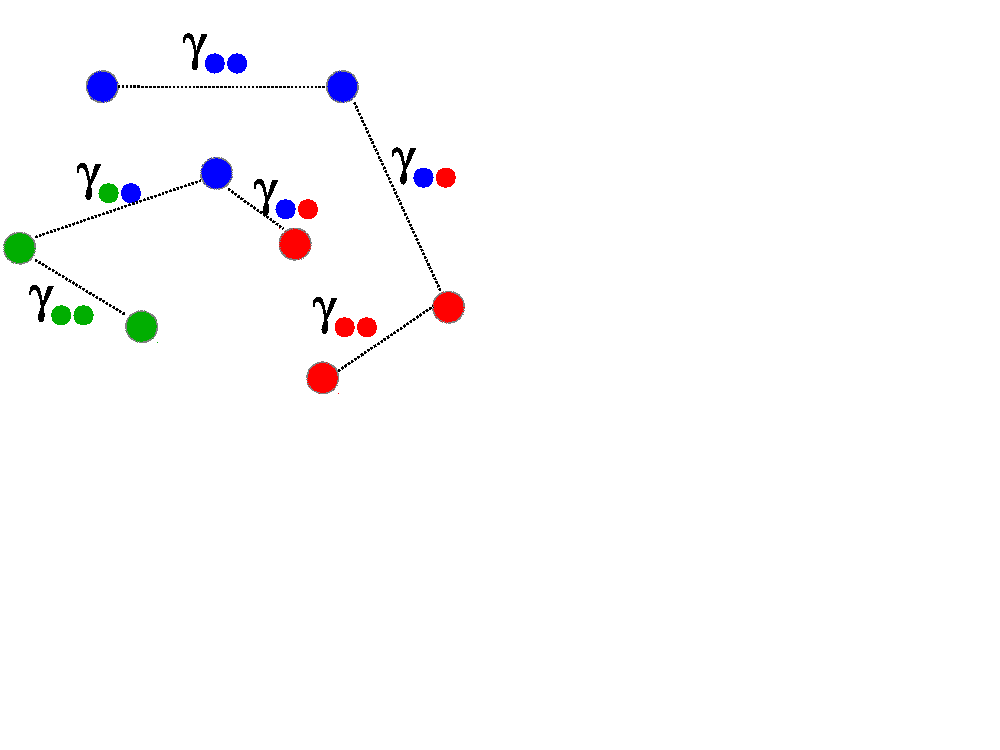
\epsfig{file = \fignet/FigSBM-Model-3.eps,
          width=.75\textwidth, clip=}    
        \onslide<5>
%        \epsfig{file = \fignet/FigSBM-Model-4.eps,
%        width=.75\textwidth, clip=}    
%        \onslide<6>
        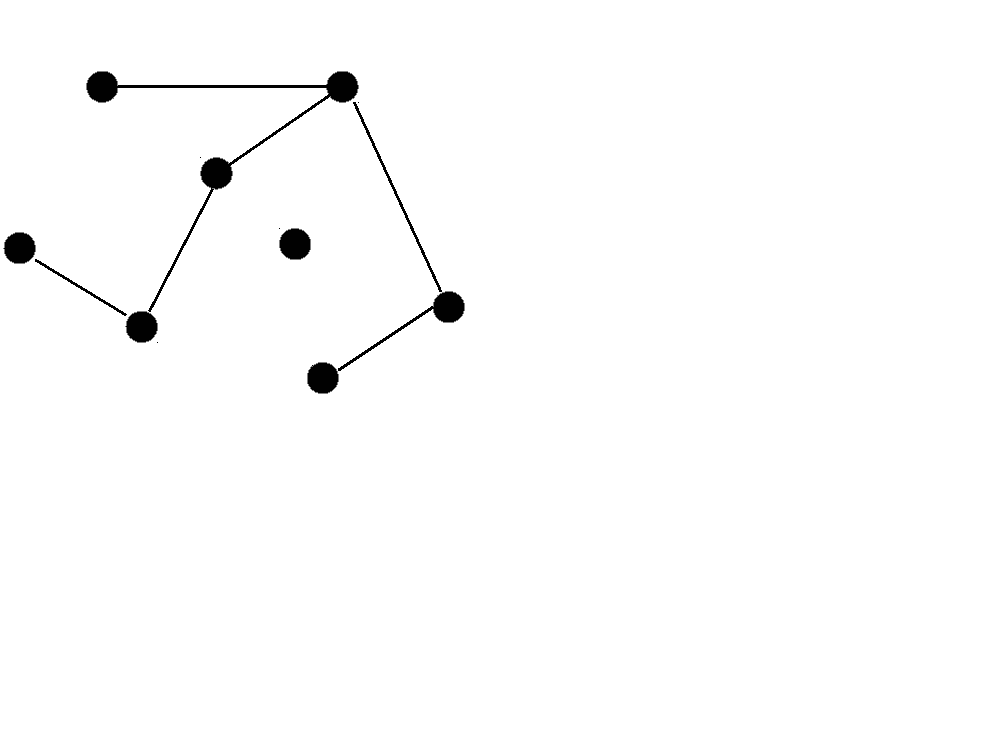
\epsfig{file = \fignet/FigSBM-Model-5.eps,
          width=.75\textwidth, clip=}    
      \end{overprint}
    \end{tabular}
  \end{tabular}
  }

%-------------------------------------------------------------------- 
\frame{ \frametitle{SBM for a binary social network}

  \vspace{-.5cm}
  \begin{tabular}{ll}
%      \paragraph{An example.}
%      & 
%      \\
      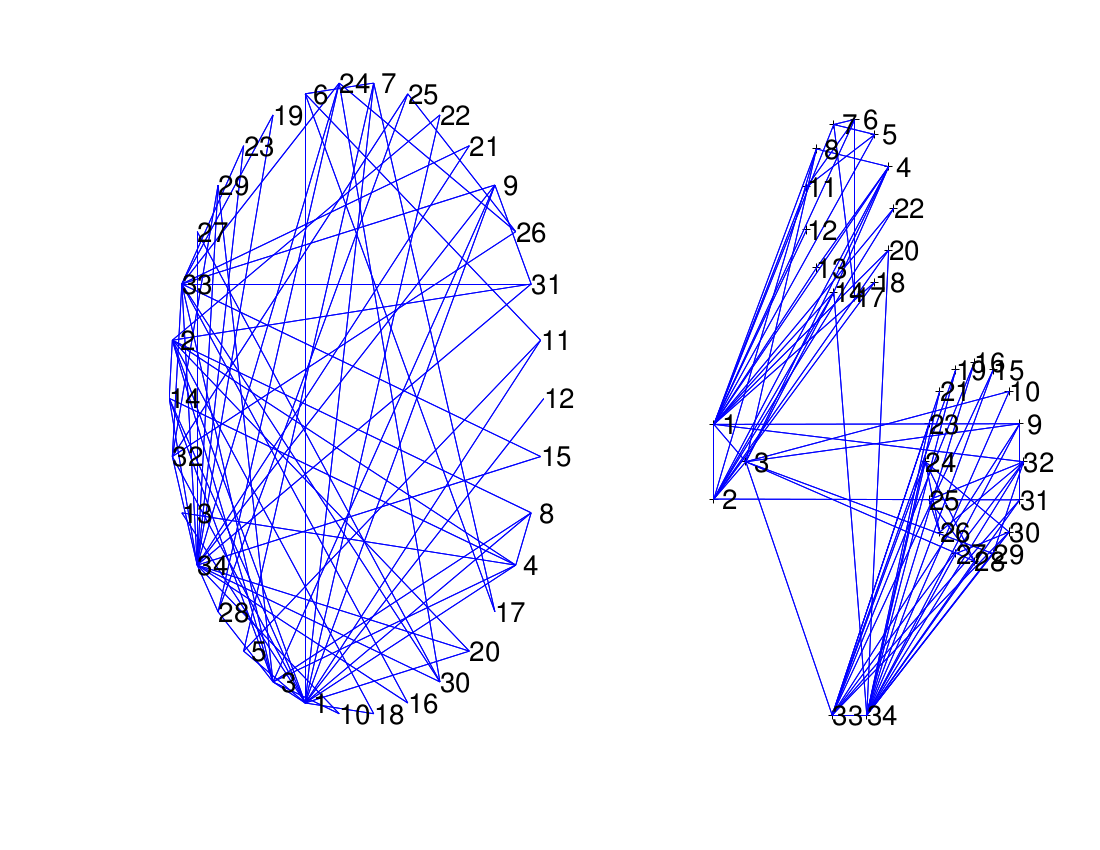
\epsfig{file = \fignet/Karate-Graph.eps, clip=, width=3.5cm,
        height=5cm, angle=270, bllx=50, bblly=80, bburx=530,
        bbury=420} 
      &
      \onslide+<2->{
        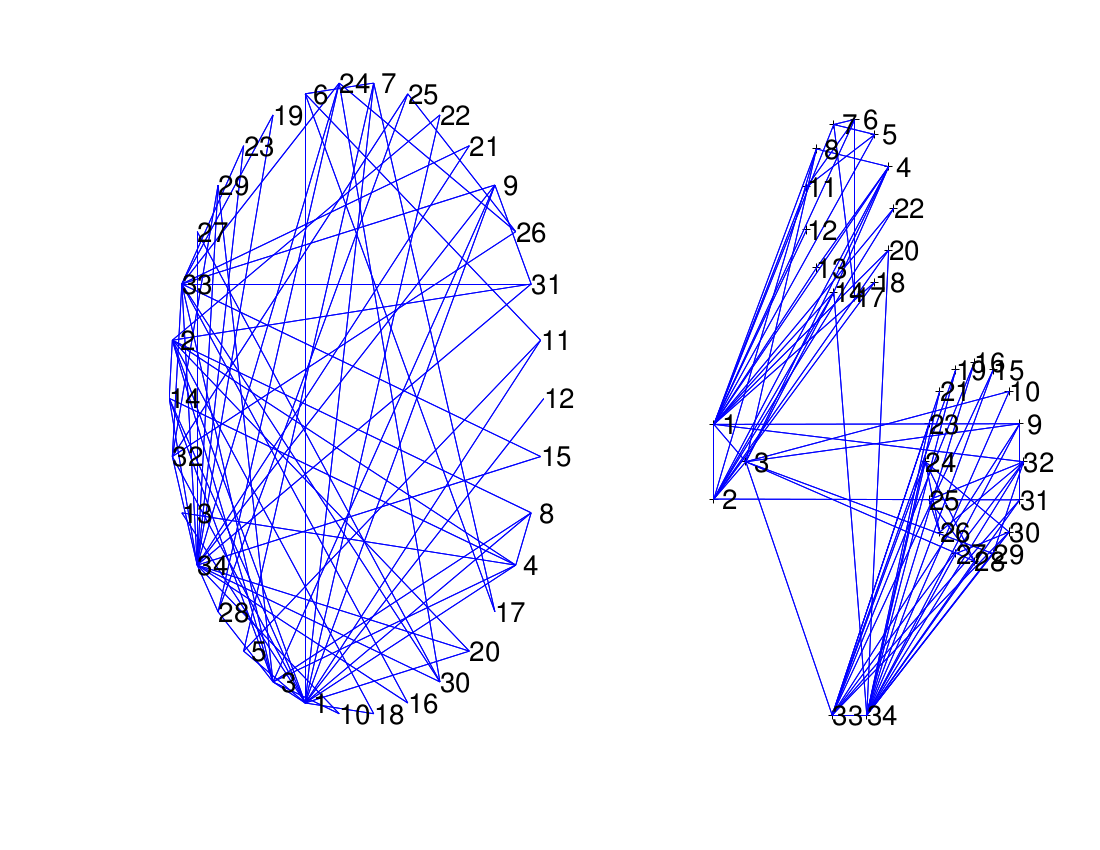
\epsfig{file = \fignet/Karate-Graph.eps, clip=, width=3.5cm,
          height=5cm, angle=270, bllx=70, bblly=490, bburx=530,
          bbury=770} 
        }
      \\     
      \medskip
      \begin{tabular}{p{.4\textwidth}}
        \paragraph{Zachary data.} Social binary network of friendship
        within a sport club. \\ 
        \\ 
        \onslide+<2->{
          \paragraph{Results.} 
          The split is recovered and the role of few leaders is
          underlined. 
          }
      \end{tabular}
      & 
      \begin{tabular}{p{.5\textwidth}}
        \onslide+<3->{
          $
          (X_{ij}|Z_i=q, Z_j=\ell) \sim \Bcal(\gamma_{q\ell})
          $ \\ ~\\
          {\small
            \begin{tabular}{c|rrrr}
              (\%) & \multicolumn{4}{c}{$\widehat{\gamma}_{k\ell}$} \\
              $k / \ell$ &  {1} & 2 & 3 &  4 \\
              \hline
              {1} &  {100} &   {53} &  {16} & {16} \\  
              {2} & - &  {12} & {0} & {7}  \\  
              3 & - & - & 8 & 73 \\
              4 & - & - & - & 100\\
              \hline
              $\widehat{\pi}_{\ell}$        & 9 &  38       & 47    & 6     \\
            \end{tabular}
            }
          }
    \end{tabular}
  \end{tabular}
}

%--------------------------------------------------------------------
\frame{\frametitle{Frequentist maximum likelihood inference}

  \begin{tabular}{cc}
    \hspace{-.5cm}
    \begin{tabular}{p{.5\textwidth}}
      \onslide+<1->{
        \paragraph{Maximum likelihood.} MLE of $\thetabf$ 
        obtained via the E-M algorithm ... \\
        provided that we can calculate
        $$
        P(\Zbf | \Xbf; \thetabf).
        $$
        ~\\~\\~\\
      }
    \end{tabular}
    & 
    \hspace{-.5cm}
    \begin{tabular}{p{.5\textwidth}}
            \begin{overprint}
        \onslide<2>
        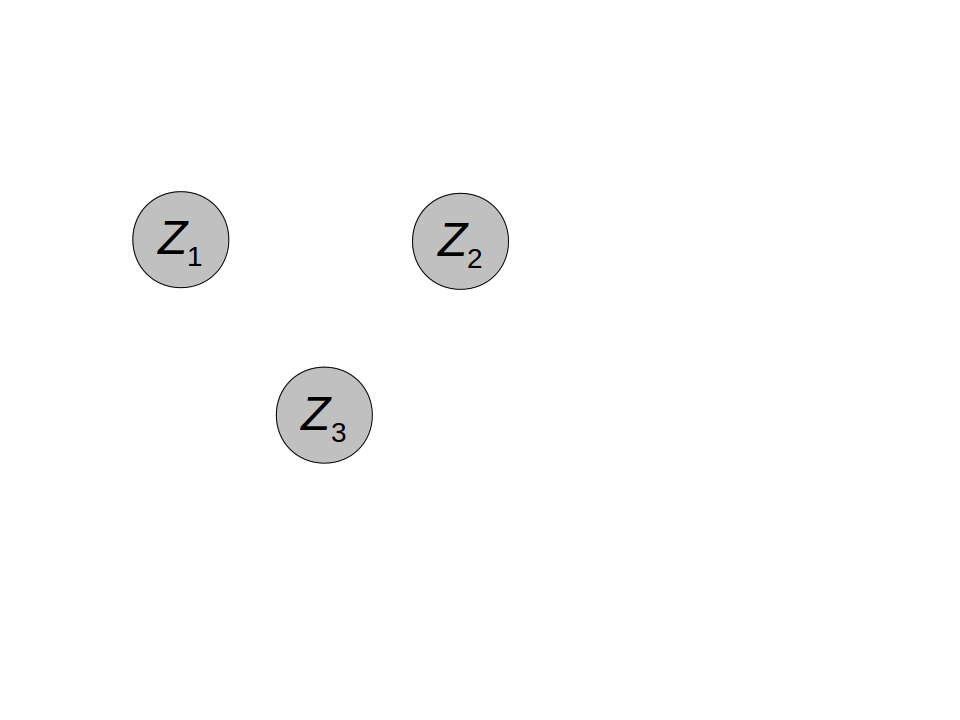
\epsfig{file=../FIGURES/FigSBM-Z.eps, clip=, width=0.6\textwidth}
        \onslide<3>
        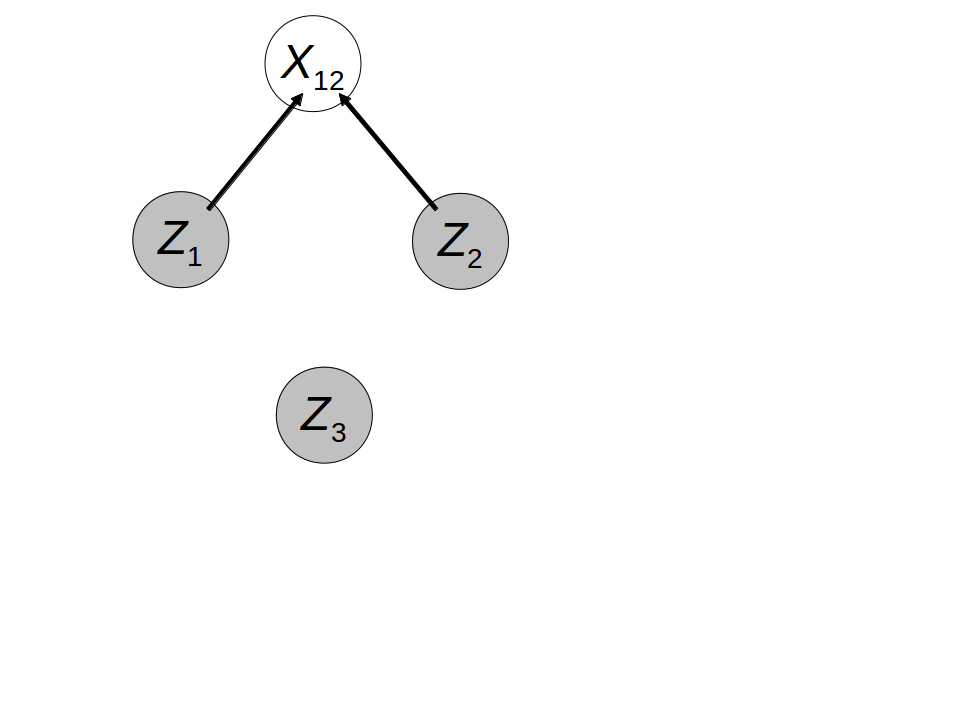
\epsfig{file=../FIGURES/FigSBM-Z-X12.eps, clip=, width=0.6\textwidth}
        \onslide<4>
        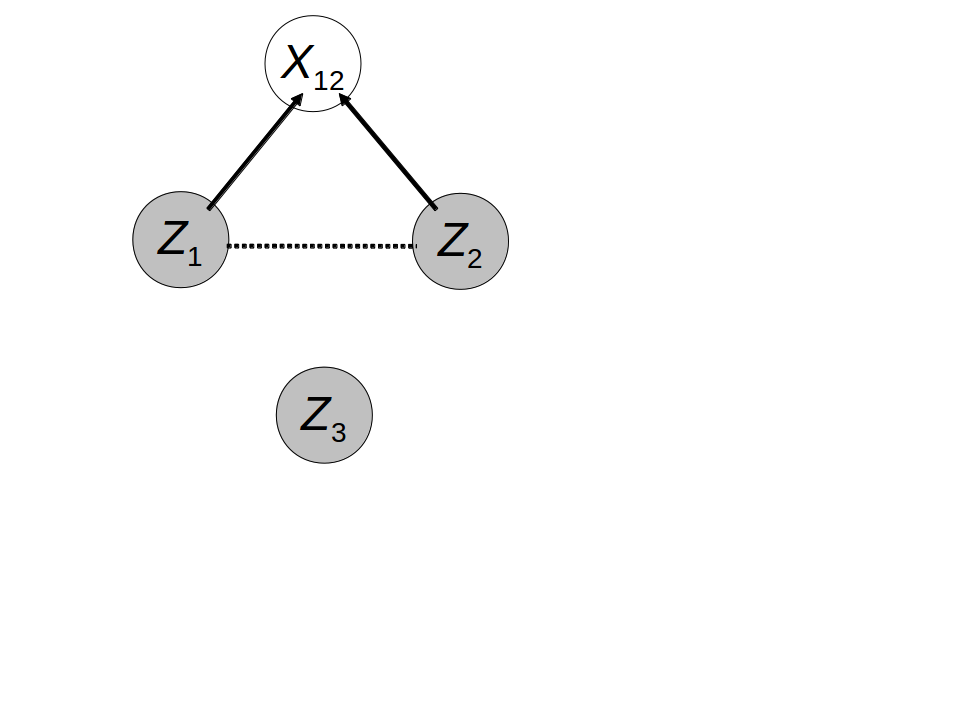
\epsfig{file=../FIGURES/FigSBM-Z-X12-Moral.eps, clip=,
          width=0.6\textwidth} 
        \onslide<5>
        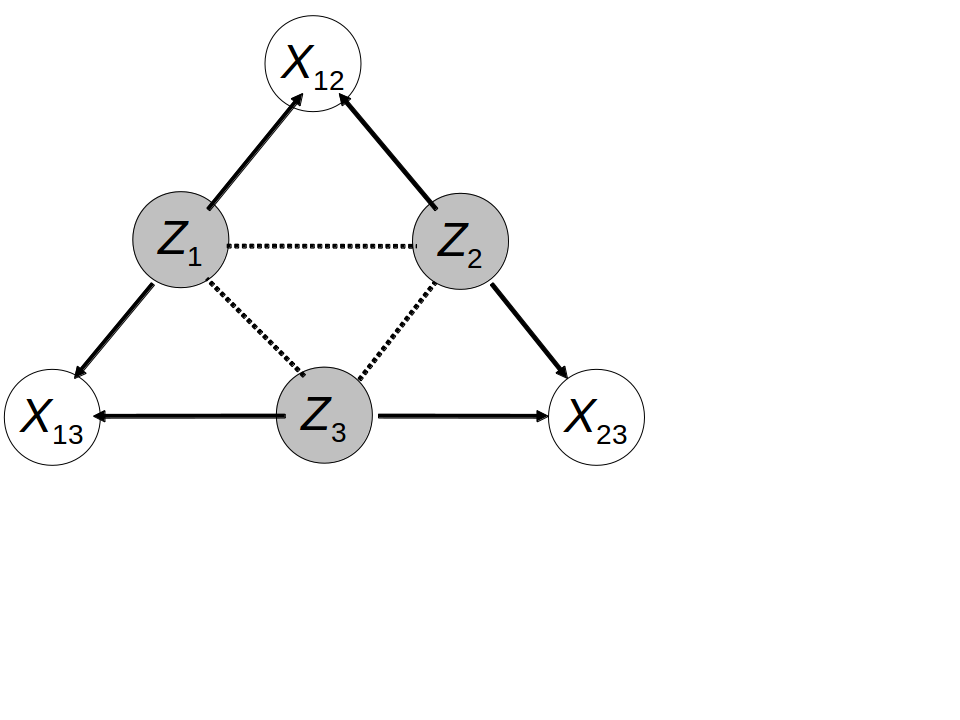
\epsfig{file=../FIGURES/FigSBM-Z-X-Moral.eps, clip=,
          width=0.6\textwidth} 
        \onslide<6->
        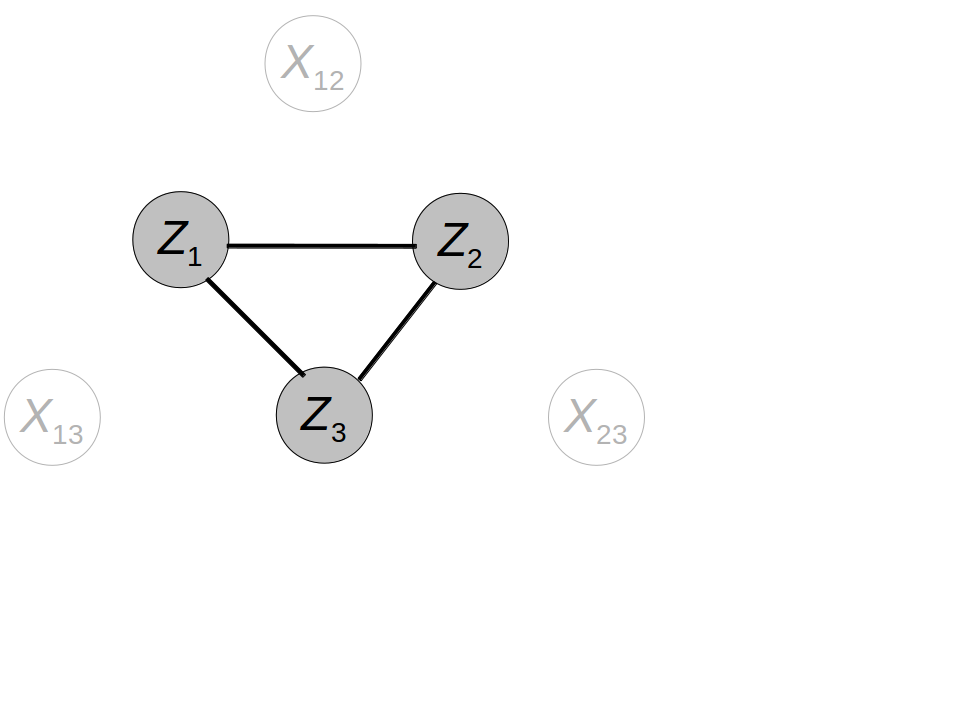
\epsfig{file=../FIGURES/FigSBM-ZcondX.eps, clip=,
          width=0.6\textwidth}
      \end{overprint}
    \end{tabular}
  \end{tabular}

  \onslide+<6->{
    \vspace{-1.5cm}
    \paragraph{Conditional distribution.} The dependency graph of
    $\Zbf$ given $\Xbf$ is a clique. \\
    \ra No factorization can be hoped (unlike for HMM). \\
    \ra $P(\Zbf | \Xbf; \thetabf)$ can not be computed
    (efficiently). \\
    \ra Variational techniques provide 
    $$
    Q(\Zbf) \simeq P(\Zbf | \Xbf).
    $$
  }
}

%--------------------------------------------------------------------
\frame{\frametitle{Bayesian inference}
  
  \begin{tabular}{cc}
    \hspace{-.5cm}
    \begin{tabular}{p{.5\textwidth}}
      We are now interested in 
      $$
      P(\Zbf, \thetabf | \Xbf)
      $$
      which is more intricate than $P(\Zbf | \Xbf; , \thetabf)$.
      \\~\\~\\~\\~\\
    \end{tabular}
    & 
    \hspace{-.5cm}
    \begin{tabular}{p{.5\textwidth}}
      \begin{overprint}
        \onslide<2>
        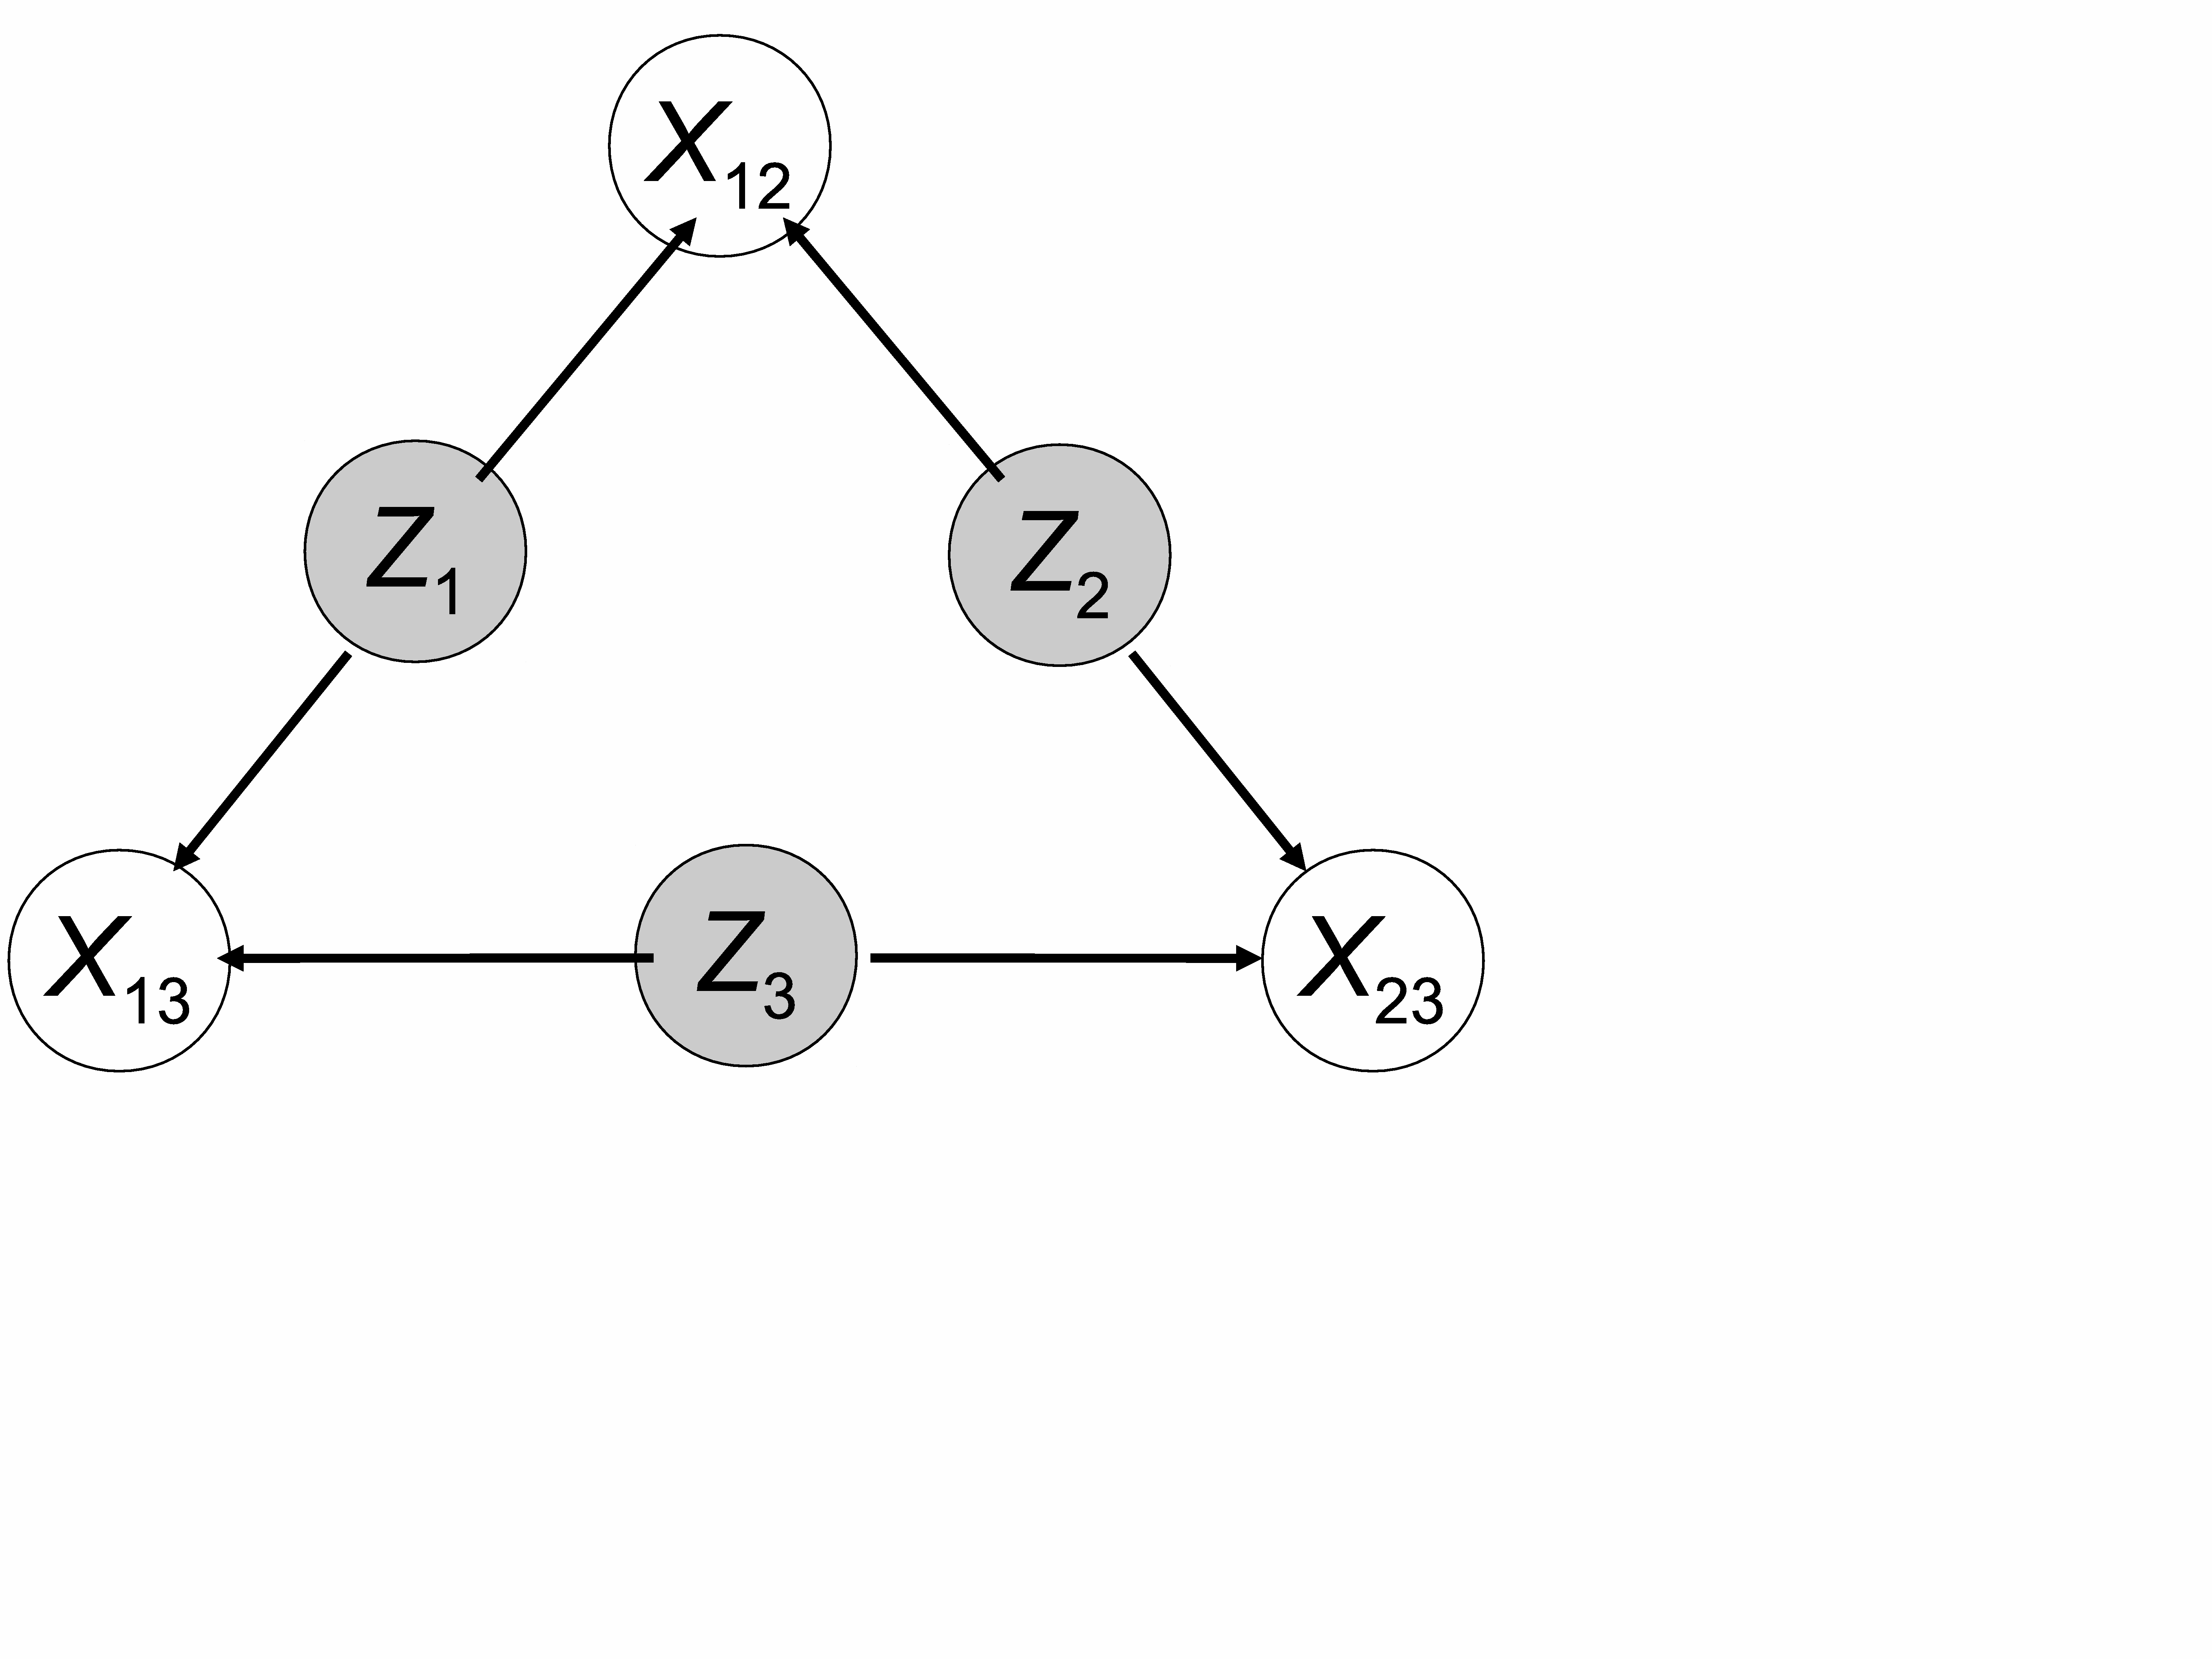
\epsfig{file = \fignet/FigSBM-Z-X.eps,
          width=.7\textwidth, clip=}   
        \onslide<3>
        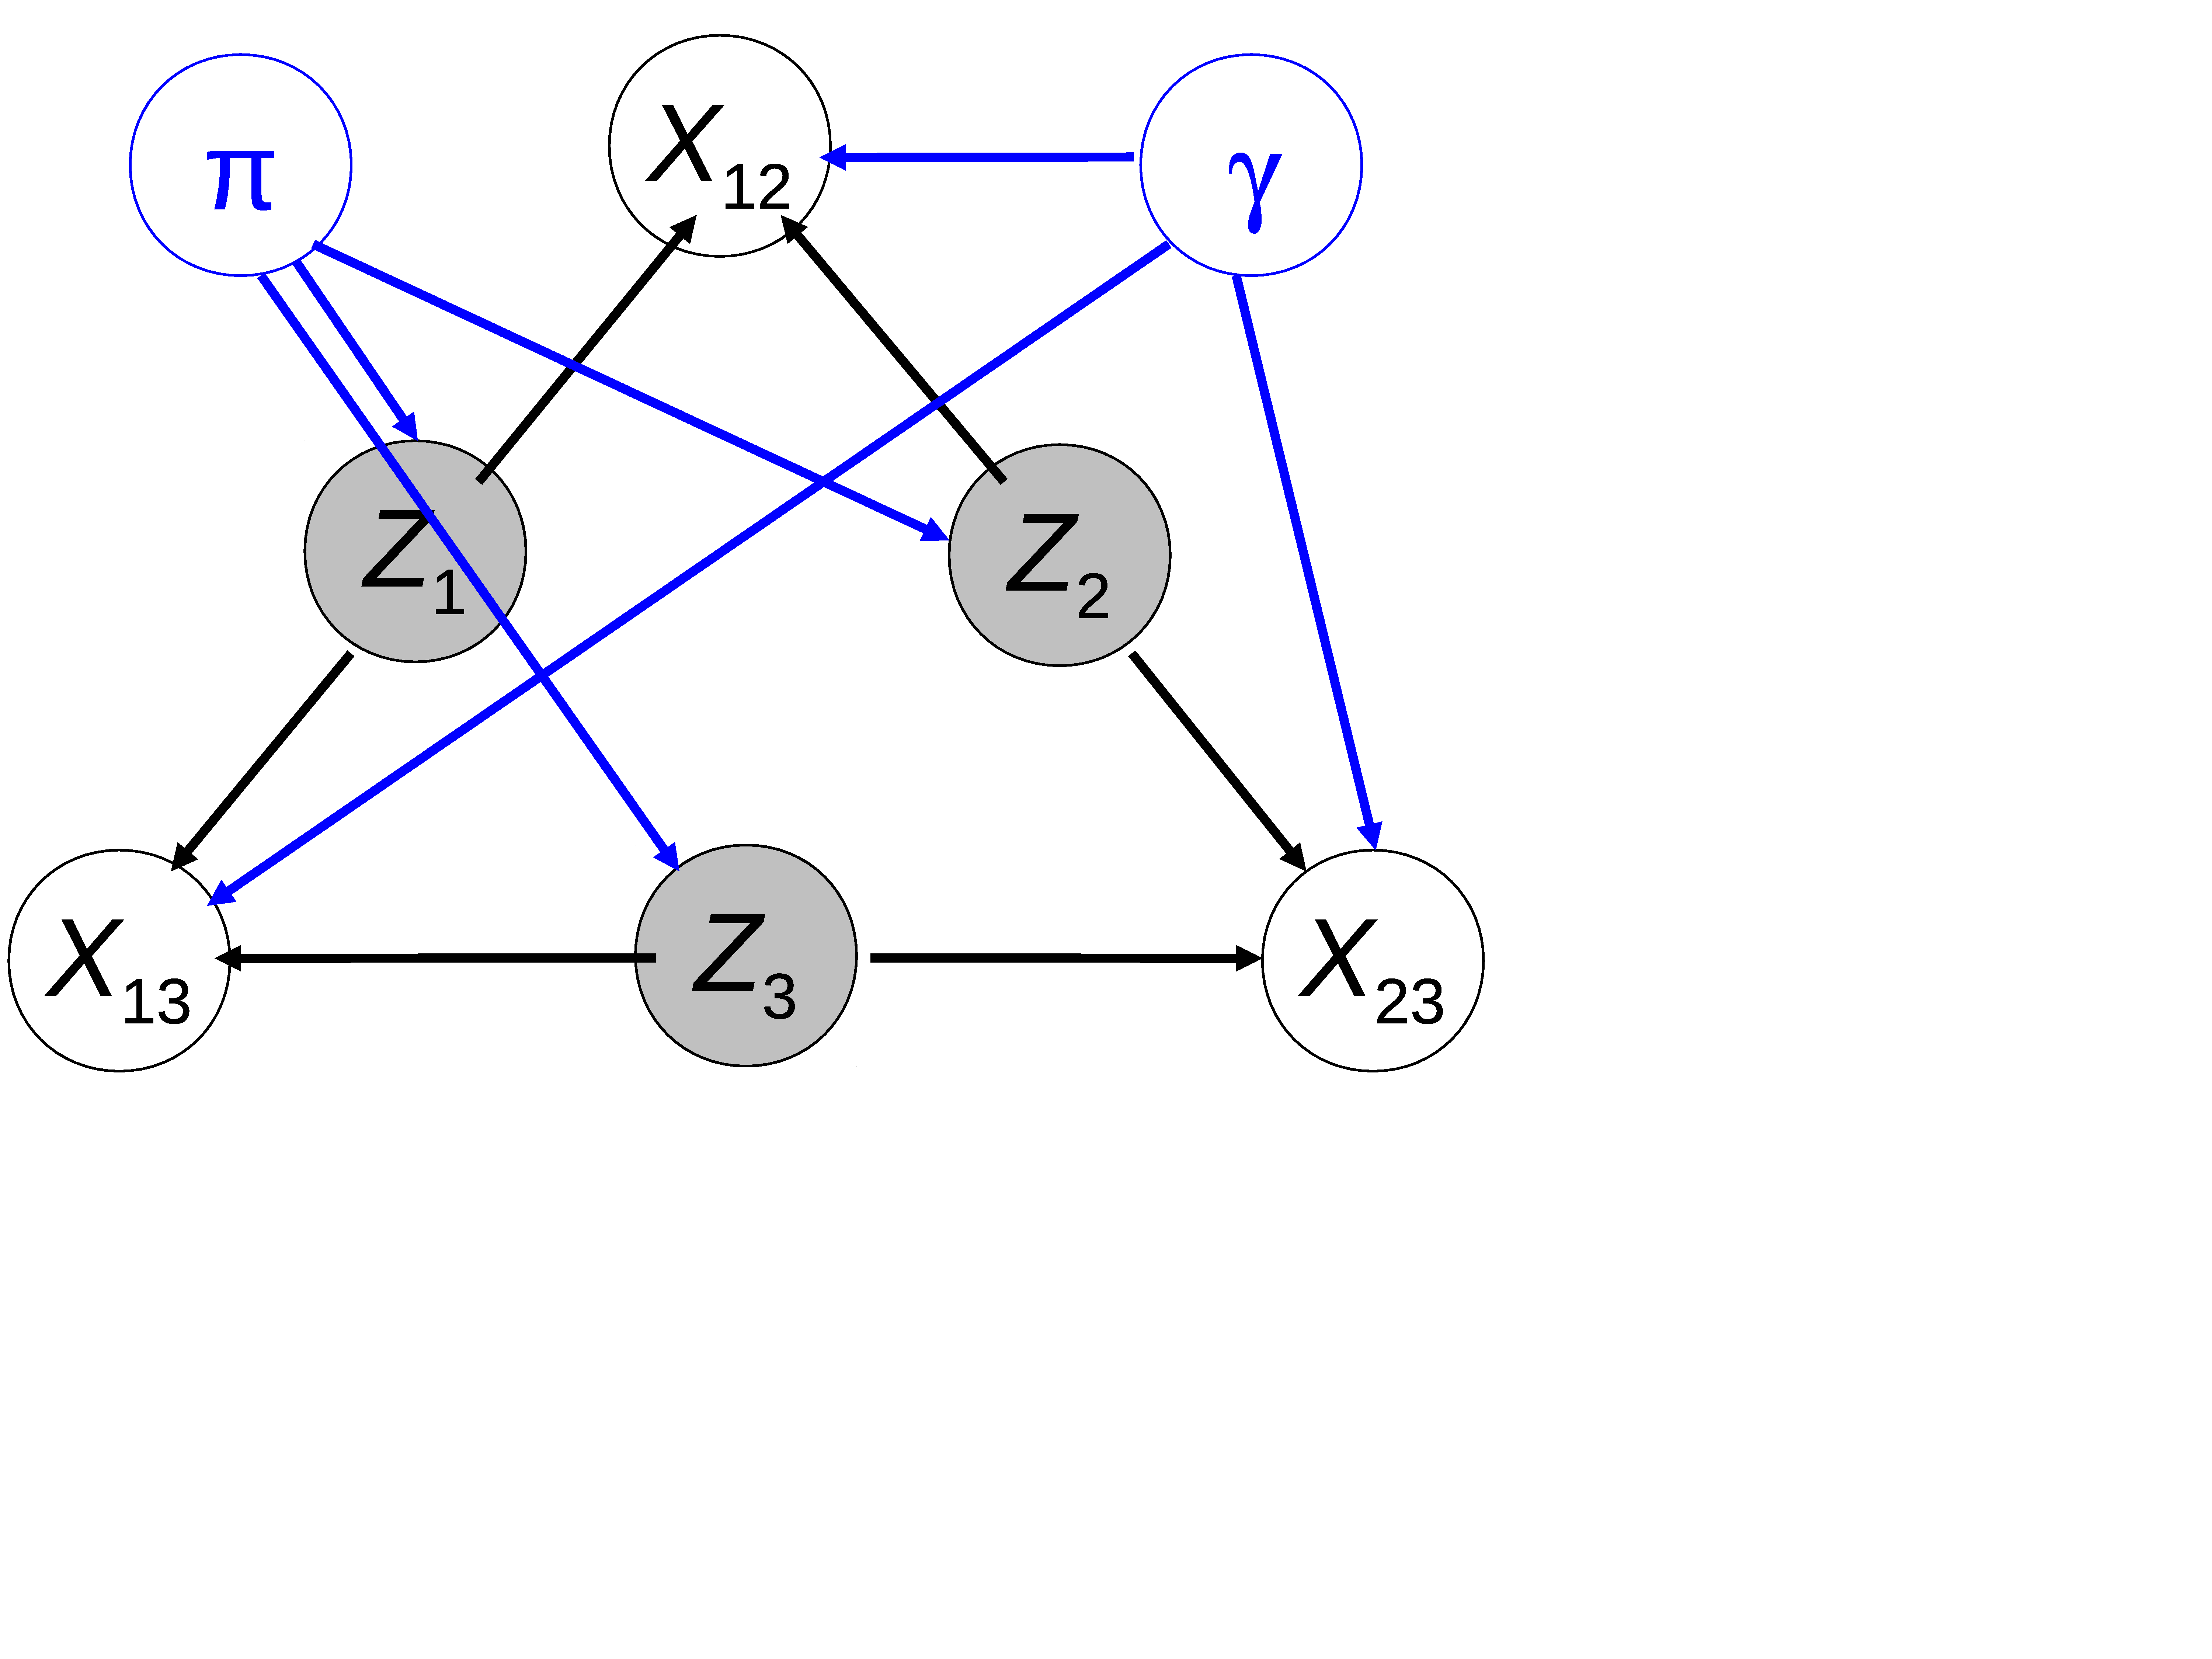
\epsfig{file = \fignet/FigSBM-Bayes-1.eps,
          width=.7\textwidth, clip=}   
        \onslide<4>
        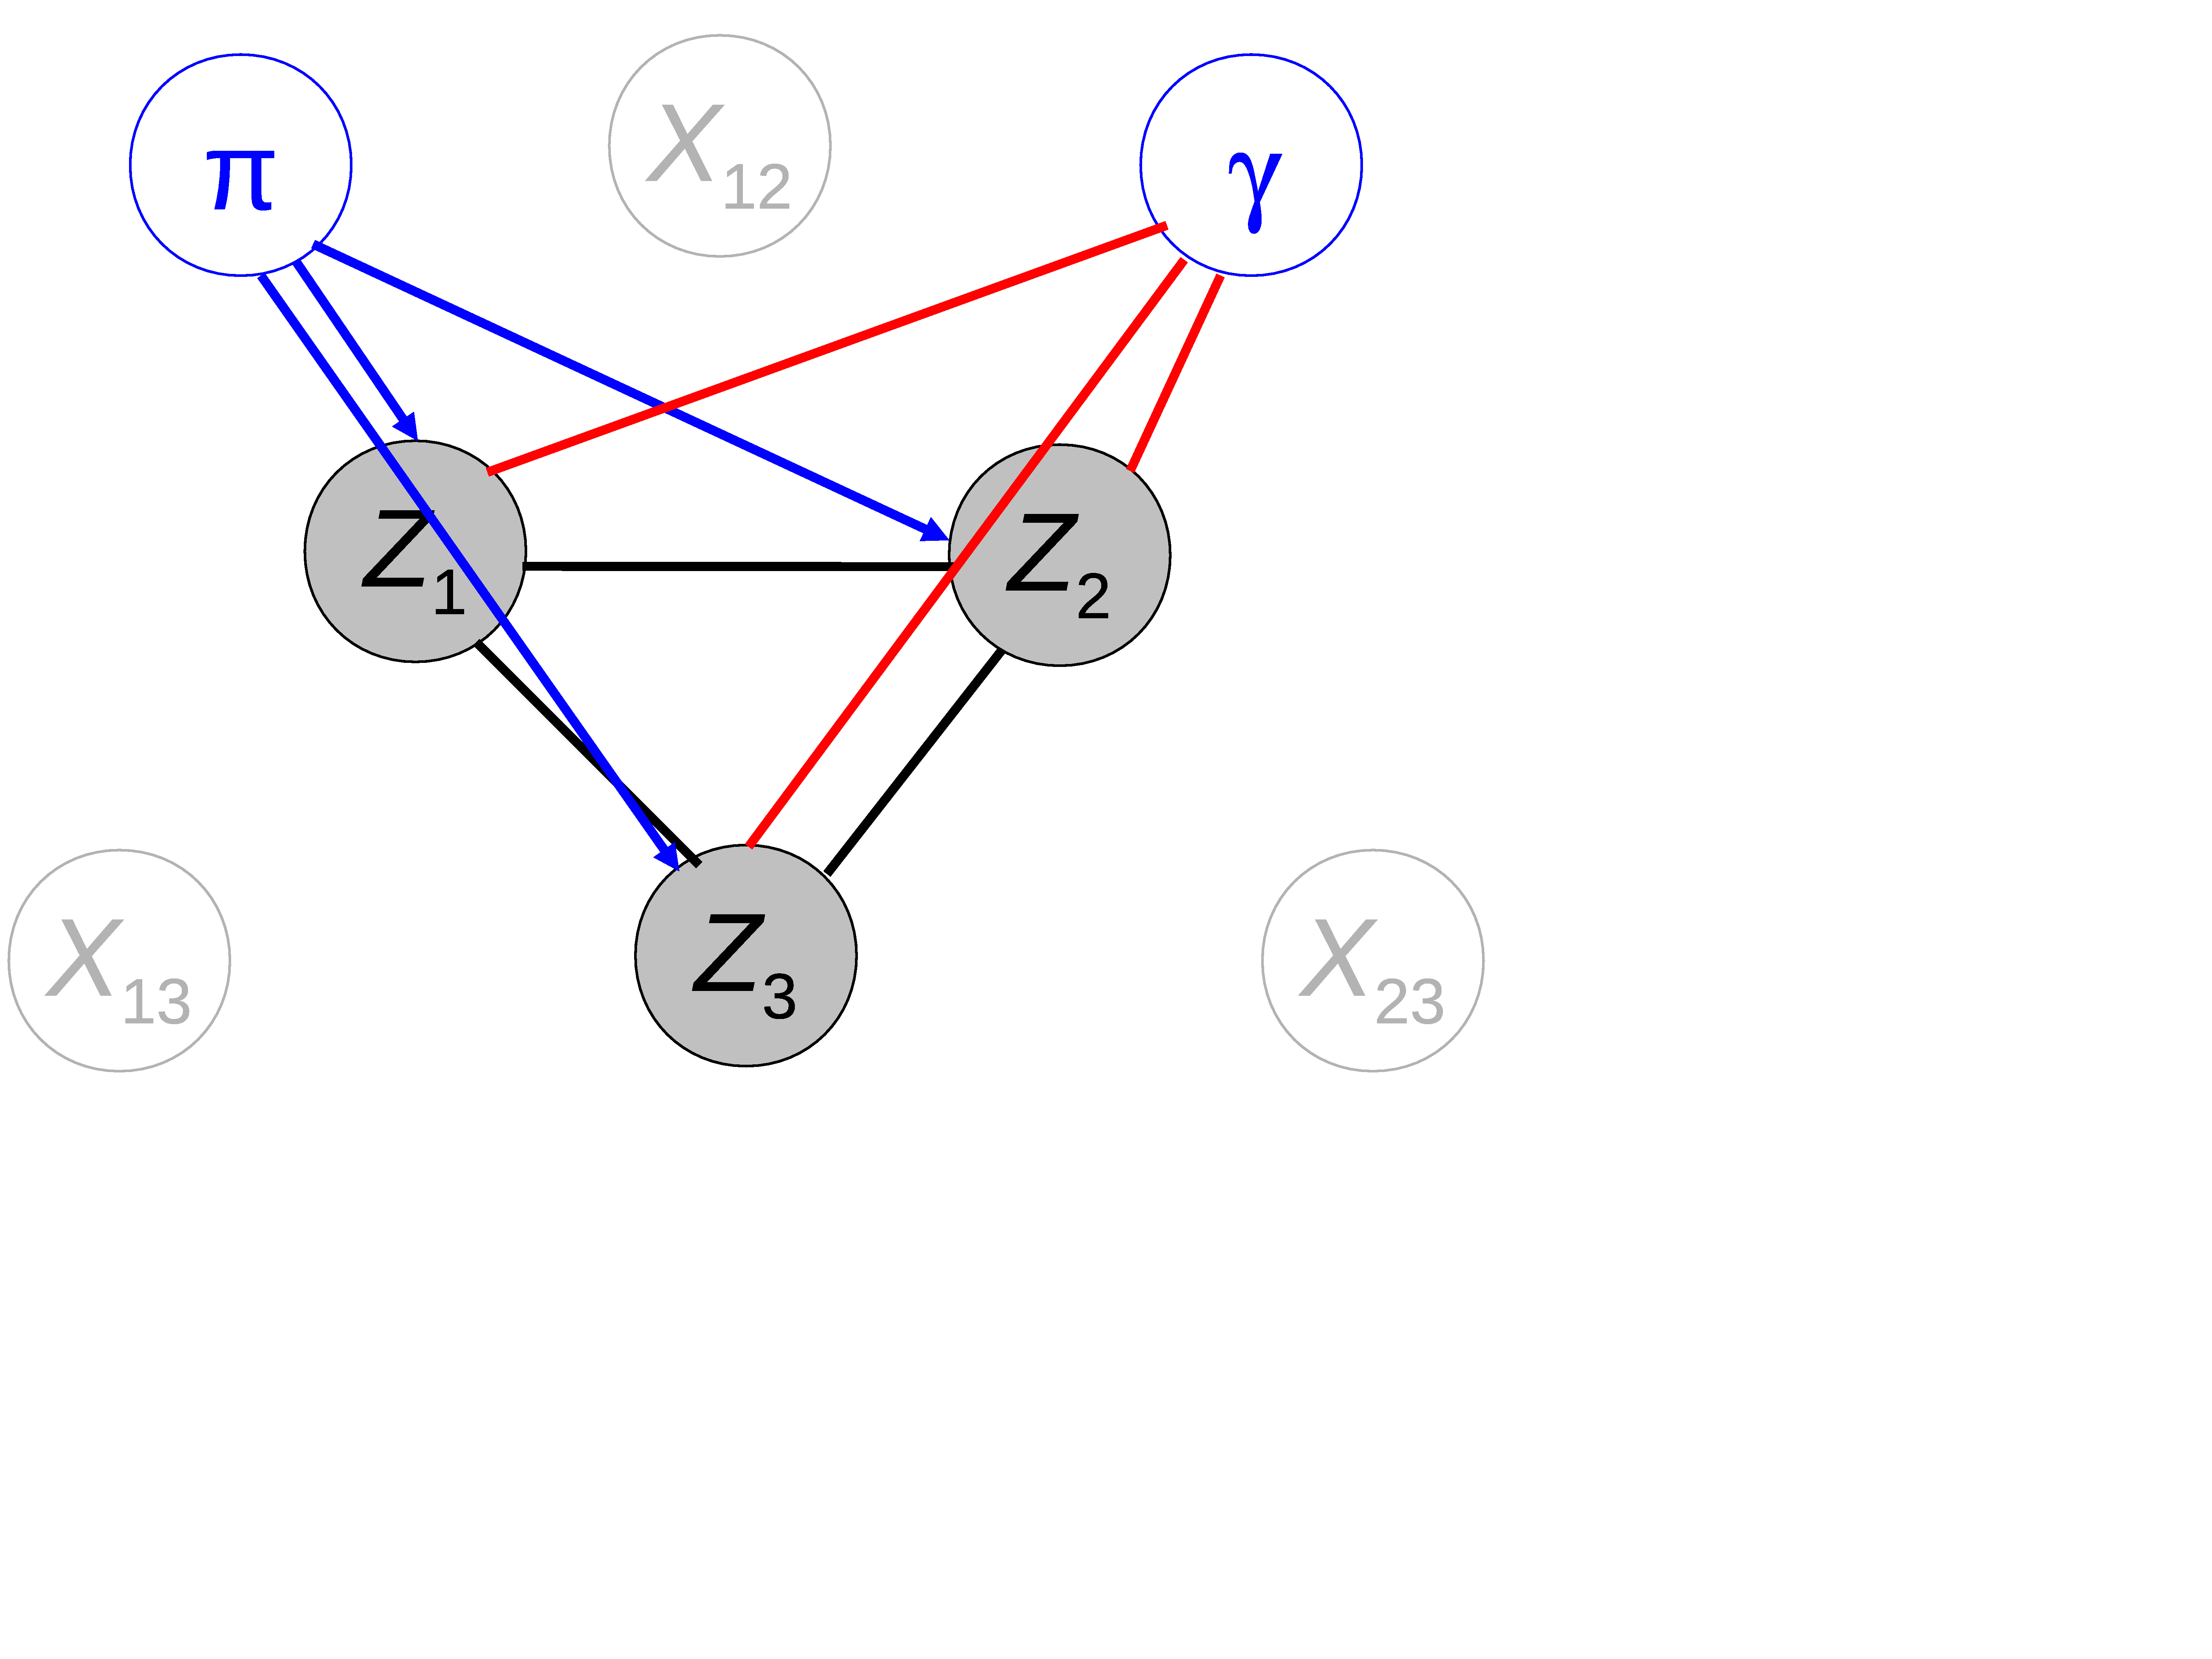
\epsfig{file = \fignet/FigSBM-Bayes-2.eps,
          width=.7\textwidth, clip=}   
      \end{overprint}
    \end{tabular}
  \end{tabular}
  
  \onslide+<4>{
    \vspace{-1cm}
    Variational techniques can provide an approximation
    $$
    Q(\Zbf, \thetabf) \simeq P(\Zbf, \thetabf | \Xbf).
    $$}
  }

%--------------------------------------------------------------------
%--------------------------------------------------------------------
\section{Variational approximation}
\frame{\frametitle{Variational approximation}}

%--------------------------------------------------------------------
\subsection*{K�llback-Leibler divergence}
%--------------------------------------------------------------------
\frame{\frametitle{K�llback-Leibler divergence}

  \paragraph{Definition.}
  \begin{eqnarray*}
    KL[Q(\cdot), P(\cdot)] & = & \int Q(\zbf) \log
    \frac{Q(\zbf)}{P(\zbf)} \dd \zbf \\
    & = & \int Q(\zbf) \log Q(\zbf) \dd \zbf - \int Q(\zbf) \log
    P(\zbf) \dd \zbf  
  \end{eqnarray*}

  \bigskip\bigskip\pause
  \paragraph{Some properties.}
  \begin{itemize}
  \item Always positive.
  \item Null iff $P = Q$.
  \item Contrast consistent with maximum-likelihood inference.
  \item Not a distance, only a 'divergence'.
  \end{itemize}
  }

%--------------------------------------------------------------------
\frame{\frametitle{Variational inference}

  \paragraph{Lower bound of the log-likelihood.} For any distribution
  $Q(\Zbf)$ \refer{Jaa00,WaJ08},
  \begin{eqnarray*}
    \log P(\Xbf) & \geq & \log P(\Xbf) - KL[Q(\Zbf),
    P(\Zbf|\Xbf)] \\ \pause
%    & = & \log P(\Xbf; \thetabf) - \int Q(\zbf) \log Q(\zbf) \dd \zbf
%    + \int
%    Q(\zbf) \log P(\zbf|\Xbf) \\
%    & = & \log P(\Xbf; \thetabf) - \int Q(\zbf) \log Q(\zbf) \dd \zbf
%    + \int
%    Q(\zbf) \log P(\Xbf, \zbf) - \int Q(\zbf) \log P(\Xbf) \dd \zbf \\ 
    & = & \int Q(\zbf) \log P(\Xbf, \zbf) \dd \zbf - \int Q(\zbf) \log
    Q(\zbf) \dd \zbf \\ \pause
    & = & \Esp_Q[\log P(\Xbf, \Zbf)] + \Hcal[Q(\Zbf)] 
  \end{eqnarray*}
  
  \bigskip\bigskip\pause
  \paragraph{Link with E-M.} This is similar to
  $$
  \log P(\Xbf) = \Esp[\log P(\Xbf, \Zbf)|\Xbf] + \Hcal[P(\Zbf | \Xbf)]
  $$
  replacing $P(\Zbf|\Xbf)$ with $Q(\Zbf)$.


  }

%--------------------------------------------------------------------
\frame{\frametitle{Variational E-M algorithms}

  \paragraph{Variational E-M.} 
  \begin{itemize}
  \item M-step: compute 
    $$
    \widehat{\thetabf} = \arg\max_\thetabf \emphase{\Esp_{Q^*}}[\log P(\Xbf,
    \Zbf; \thetabf)].
    $$
  \item \pause E-step: replace the calculation of $P(\Zbf|\Xbf)$ with
    the search of
    $$
    Q^*(\Zbf) = \emphase{\arg\min_{Q \in \Qcal} KL}[Q(\Zbf), P(\Zbf|\Xbf)].
    $$
  \end{itemize}
  
  \bigskip\pause
  \paragraph{Variational Bayes E-M.} Directly search for
  $$
  Q^*(\Zbf, \thetabf) = \emphase{\arg\min_{Q \in \Qcal} KL}[Q(\Zbf, \thetabf),
  P(\Zbf, \thetabf|\Xbf)].
  $$
  }

%--------------------------------------------------------------------
\subsection*{A functional optimization problem}
%--------------------------------------------------------------------
\frame{\frametitle{A functional optimization problem}

  We want to minimize, \emphase{with respect to the function $Q$}, the
  functional
  $$
  \Fcal(\emphase{Q}) = \int \Lcal[\emphase{Q}(\zbf), \zbf] \dd \zbf.
  $$
  
  \pause\bigskip
  \paragraph{Example.} For variational inference, take either $\zbf =
  \zbf$ or $\zbf = (\zbf, \thetabf)$ and set
  $$
  % \Lcal[Q(\zbf), \zbf] = Q(\zbf) \log\frac{Q(\zbf)}{P(\zbf|\Xbf)}, 
  \Lcal[\emphase{Q}(\zbf), \zbf] = \emphase{Q}(\zbf)
  \log\left[\emphase{Q}(\zbf) / P(\Xbf, \zbf) \right].
  $$
  
  \bigskip\pause
  \paragraph{Theorem.} The function 
  $$
  Q^* = \arg\min_Q \Fcal(Q)
  $$ 
  satisfies
  $$
  \forall \zbf, \qquad \left. \frac{\partial \Lcal[Q(\zbf),
      \zbf]}{\partial Q(\zbf)} \right|_{\emphase{Q^*}(\zbf)}= 0.
  $$

  }

%--------------------------------------------------------------------
\frame{\frametitle{Sketch of proof}

  \begin{enumerate}
  \item \pause $Q^*$ is optimal if, \emphase{for any function $H$}
    ('perturbation', 'direction'),
    $$
    \left. \frac{\partial}{\partial t} \Fcal(Q^* +tH)\right|_{t = 0} = 0.
    $$ ~\\
  \item \pause At \emphase{$t=0$}, under regularity conditions (and
    since $(f \circ g)' = g' \times f' \circ g$)
    $$
    \frac{\partial}{\partial t} \Fcal(Q +tH) 
    = \int \frac{\partial}{\partial t} \Lcal[Q(\zbf)+tH(\zbf), \zbf]
    \dd \zbf 
    = \int H(\zbf) \frac{\partial \Lcal[Q(\zbf), \zbf]}{\partial
      Q(\zbf)} \dd \zbf.
    $$ ~\\
  \item \pause The '\emphase{fundamental lemma} of variation calculus'
    says that
    $$
    \forall h, \; \int f(\zbf) h(\zbf) \dd \zbf = 0  \qquad
    \Rightarrow \qquad \forall \zbf, \; f(\zbf) = 0.
    $$
  \end{enumerate}
  }

%--------------------------------------------------------------------
\frame{\frametitle{Some remarks}

  \begin{itemize}
  \item \pause A constraint can be added to guaranty that $Q(\zbf)$ is a
    distribution:
    $$
    \Fcal(Q) = \int \Lcal[Q(\zbf), \zbf] \dd \zbf - \lambda \left[\int
      Q(\zbf) \dd \zbf - 1\right].
    $$ ~\\
  \item \pause The solution of $\min_Q KL[Q(\Zbf), P(\Zbf|\Xbf)]$ is
    \emphase{actually known}:
    $$
    \arg\min_Q KL[Q(\Zbf), P(\Zbf|\Xbf)] = P(\Zbf|\Xbf) \quad ...
    $$ ~\\
  \item \pause That's why we need to restrict the problem:
    $$
    \arg\min_{\emphase{Q \in \Qcal}} KL[Q(\Zbf), P(\Zbf|\Xbf)]
    $$
    where $\Qcal$ is a class of \emphase{'nice' distributions}.
  \end{itemize}
  
  }

%--------------------------------------------------------------------
%--------------------------------------------------------------------
\section{Variational inference}
\frame{\frametitle{Variational inference}}
%--------------------------------------------------------------------
\subsection*{Variational E-M for SBM}
%--------------------------------------------------------------------
\frame{\frametitle{Stochastic Block Model (SBM)}

  \paragraph{Likelihoods.} $Z_i =$ label, $X_{ij} = $ edge, $\thetabf
  = (\pibf, \gammabf)$
  \begin{eqnarray*}
    P(\Zbf) & = & \prod_i \prod_k \pi_k^{\emphase{Z_{ik}}}  \qquad\qquad \text{where }
    Z_{ik} = \Ibb\{i \in k\}, \\
    P(\Xbf | \Zbf) & = & \prod_{i \neq j} \prod_{k, \ell}
    \underset{f_{k\ell}(X_{ij})}{\underbrace{\left[\gamma_{k\ell}^{X_{ij}}
          (1 - \gamma_{k\ell})^{1-
            X_{ij}}\right]}}^{\emphase{Z_{ik}Z_{j\ell}}}.  
  \end{eqnarray*}
  \ra We only need $P(Z_i |\Xbf)$ and $P(Z_i, Z_j|\Xbf)$.

  \bigskip\bigskip\pause
  \paragraph{Remark.} The conditional distribution of one label given
  the data \emphase{+ all other labels} is
  \begin{eqnarray*}
%    P(Z_i | \Xbf) & \propto & \sum_{\{Z_j\}_{j \neq i}}P(Z_i,
%    \{Z_j\}_{j \neq i}, \Xbf) \quad ... \\
    P(Z_i = k | \Xbf, \{Z_j\}_{j \neq i}) & \propto &  \pi_k \prod_{j
    \neq i} \prod_\ell f_{k\ell}(X_{ij})^{\emphase{Z_{j\ell}}}
  \end{eqnarray*}
  }

%-------------------------------------------------------------------- 
\frame{ \frametitle{Variational E-M}

  \paragraph{Distribution class.} $\Qcal =$ set of \emphase{factorisable}
  distributions:
  $$
  \Qcal = \{Q: Q(\Zbf) = \prod_i Q_i(Z_i)\}, \qquad\qquad Q_i(Z_i) = \prod_k
  \tau_{ik}^{Z_{ik}}.
  $$
  \ra The approximate joint distribution is $Q(Z_i, Z_j) = Q_i(Z_i)
  Q_j(Z_j)$. 

  \bigskip\bigskip\bigskip\pause
  Applying the theorem (or directly minimizing $\Fcal(Q)$) leads to
  \emphase{fix-point} relation:
  $$
  \tau_{ik} \propto \pi_k \prod_{j \neq i} \prod_\ell
  f_{k\ell}(X_{ij})^{\emphase{\tau_{j\ell}}}
  $$
  also known as  \emphase{mean-field approximation} in physics. \refer{DPR08}
  }

%-------------------------------------------------------------------- 
\frame{ \frametitle{Application to a regulatory network}
  \vspace{-.5cm}\hspace{-.5cm}
  \begin{tabular}{ll}
    \begin{tabular}{p{6.1cm}}
      \paragraph{Regulatory network =} directed graph 
      \begin{itemize}
      \item \emphase{Nodes =} genes (or groups of genes, e.g. operons)
      \item \emphase{Edges =} regulations:
        $$
        \emphase{\{i \rightarrow j\}}
        \quad \Leftrightarrow \quad 
        \emphase{i \text{ regulates } j}
        $$
      \end{itemize}

      \onslide+<3->{
        \bigskip
        \paragraph{Questions}
        \begin{itemize}
        \item Do some nodes share similar connexion profiles?
        \item Is there a 'macroscopic' organisation of the network?
        \end{itemize}    
        }
    \end{tabular}
    &
    \begin{tabular}{l}
      \onslide+<2->{
        \hspace{-1cm}
        \epsfig{file=\fignet/im_EcoliVEM_NB.ps,
          width=.45\textwidth, clip=} 
        }
    \end{tabular}
  \end{tabular}
  }

%-------------------------------------------------------------------- 
\frame{ \frametitle{SBM analysis}

  \vspace{-0.5cm}
  \hspace{-0.5cm}
  \begin{tabular}{cc}      
    \begin{tabular}{p{0.45\textwidth}}
      \paragraph{Parameter estimates.} $K = 5$     \\
      \tiny{$\begin{array}{cccccc}
          \widehat{\gamma}_{k\ell}~(\%) & 1 & 2 & 3 & 4 & 5 \\
          \hline
          1 & . & . & . & . & . \\
          2 & 6.40 & 1.50 & 1.34 & . & . \\
          3 & 1.21 & . & . & . & . \\
          4 & . & . & . & . & . \\
          5 & 8.64 & 17.65 & . & 72.87 & 11.01 \\
          \hline
          \widehat{\pi}~(\%) & 65.49 & 5.18 & 7.92 & 21.10 & 0.30
        \end{array}$}
      \\ ~\\

      \onslide+<3->{
        \paragraph{Meta-graph representation.} \\
        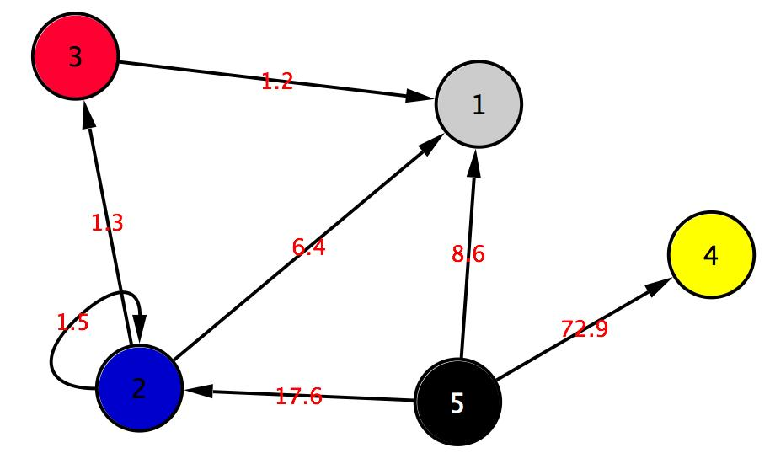
\epsfig{file=\fignet/VEMmetagraphe.ps,
          width=.4\textwidth, clip=}  \\
        }
      \\ 
      \refer{PMD09}
    \end{tabular}
    &
    \begin{tabular}{p{0.45\textwidth}}
      \onslide+<2->{
        \epsfig{file=\fignet/im_EcoliVEM_2.ps,
          width=.45\textwidth, clip=} 
        }
    \end{tabular}
  \end{tabular}
  }

%--------------------------------------------------------------------
\frame{\frametitle{Properties of the variational approximation}

  \emphase{Not much is known} about the quality of variational
  inference.
  \begin{itemize}
  \item VEM algorithm converges to a \emphase{different optimum than
      ML}, except for \emphase{'degenerated' models} \refer{GuB05}.
  \item Mean field approximation is asymptotically exact for models
    with infinite range dependency \refer{OpW01}.
  \end{itemize}

  \bigskip\bigskip\pause
  \paragraph{Specific case of graphs.}
  \begin{itemize}
  \item Specific asymptotic framework: \emphase{$n^2$ data, $'p' = n$
      'variables'} per individual.
  \item $P(\Zbf|\Xbf)$ concentrates towards a Dirac mass when $n
    \rightarrow \infty$ \refer{CDP11}.
  \item The Dirac mass belongs to $\Qcal$...
  \end{itemize}
  }

%--------------------------------------------------------------------
%--------------------------------------------------------------------
\section{Variational Bayes inference}
\frame{\frametitle{Variational Bayes inference}}
%--------------------------------------------------------------------
\subsection*{Variational Bayes E-M}
%--------------------------------------------------------------------
\frame{\frametitle{Variational Bayes inference}

  \paragraph{Exponential family / conjugate prior setting.}
  \begin{itemize}
  \item If the joint distribution $P(\Xbf, \Zbf|\thetabf)$ is in the
    exponential family
    $$
    P(\xbf, \zbf | \thetabf) \propto \exp\{\emphase{\phibf}(\thetabf)^{\transp}
    \emphase{\ubf}(\xbf, \zbf)\};
    $$
  \item If the prior distribution of $\thetabf$ is conjugate
  \begin{eqnarray*}
    P(\thetabf) & \propto & \exp\{\phibf(\thetabf)^{\transp} \emphase{\nubf}\}
    \\    \pause 
    \Rightarrow P(\xbf, \zbf, \thetabf) & \propto &
    \exp\{\phibf(\thetabf)^{\transp} [\ubf(\xbf, \zbf) + \nubf]\};
  \end{eqnarray*}
  \end{itemize}

  \bigskip\pause
  \paragraph{Class of approximate distributions.}
  \begin{itemize}
  \item If we restrict the approximate distribution $Q(\Zbf,
    \thetabf)$ to
    $$
    Q \in \Qcal = \{Q(\Zbf, \thetabf) = \QZ(\Zbf)  \Qt(\thetabf)\};
    $$
  \end{itemize}
  }

%--------------------------------------------------------------------
\frame{\frametitle{Variational optimization}

  We want to minimize $KL[Q(\Zbf, \thetabf), P(\Zbf, \thetabf |
  \Xbf)]$ \emphase{within $\Qcal$}, that is
  $$
  \Fcal(\QZ, \Qt) = \int \int \QZ(\zbf) \Qt(\thetabf) \log
  \frac{\QZ(\zbf) \Qt(\thetabf)}{P(\Xbf, \zbf, \thetabf)} \dd \zbf \dd
  \thetabf.
  $$

  \bigskip\pause
  To get the optimal $\QZ^*$, we set
  $$
  \Lcal_\Zbf[\emphase{\QZ}(\zbf), \zbf] = \emphase{\QZ}(\zbf) \int
  \Qt(\thetabf) \log \frac{\emphase{\QZ}(\zbf) \Qt(\thetabf)}{P(\Xbf, \zbf,
    \thetabf)} \dd \thetabf.
  $$

  \bigskip\pause 
  According to the theorem, $\QZ^*$ satisfies
  $$
  \frac{\partial \Lcal_\Zbf[\emphase{\QZ}(\zbf), \zbf]}{\partial
    \emphase{\QZ}(\zbf)} = \int \Qt(\thetabf) \log
      \frac{\Qt(\thetabf)}{P(\Xbf, \zbf, \thetabf)} \dd \thetabf +
      \log \emphase{\QZ}(\zbf) - 1 = 0
  $$
  }

%--------------------------------------------------------------------
\frame{\frametitle{Variational Bayes E-M algorithm}

  \paragraph{VB E-step.} The optimal $\QZ^*$ is therefore \refer{BeG03}
  \begin{eqnarray*}
    \log \QZ^*(\zbf) & = & \int \Qt(\thetabf) \log P(\Xbf, \zbf,
    \thetabf) \dd \thetabf +  \cst  \\ \pause
    & =  & \emphase{\Esp_{Q_\thetabf}}[\log P(\Xbf, \zbf, \thetabf)] + \cst \\
    \\ \pause
    \text{that is} \qquad 
    \QZ^*(\zbf) & \propto & \exp
    \left\{\emphase{\overline{\phibf}}^\transp \ubf(\Xbf,
      \zbf) \right\} \\ 
    \\ \pause
    \text{where} \qquad 
    \overline{\phibf} & = &
    \emphase{\Esp_{Q_\thetabf}}[\phibf(\thetabf)].  
  \end{eqnarray*}

  \bigskip\bigskip\pause
  \paragraph{VB E-step.} A symmetric reasoning leads to the optimal
  $\Qt^*$:
  $$
  \Qt^*(\thetabf) \propto \exp \left\{\phibf(\thetabf)^\transp
    \left[\emphase{\overline{\ubf}}(\Xbf) + \nubf\right] \right\},  
  \qquad 
  \overline{\ubf}(\Xbf) = \emphase{\Esp_{Q_\Zbf}}[\ubf(\Xbf, \Zbf)]. 
  $$
  }

%--------------------------------------------------------------------
\frame{\frametitle{Example: Poisson mixture}

  \paragraph{Model.} \hspace{3cm}
  $
  \{X_i\} \text{ i.i.d } \sim \sum_k \pi_k \Pcal(\gamma_k).
  $ \pause
  
  \bigskip
  \paragraph{Likelihood.} 
  $$
  \begin{array}{rcrcccl}
    \log P(\Xbf, \Zbf | \thetabf) & = & & \sum_{ik} Z_{ik} \log \pi_k
    & + \sum_{ik} Z_{ik} X_i \log \gamma_k & - \sum_{ik} Z_{ik}
    \gamma_k \\ \pause
    \phibf(\thetabf) & = & [ & \log\pi_k & \log \gamma_k &
    -\gamma_k & ], \\ \pause
    \ubf(\Xbf, \Zbf) & = & [ & \sum_i Z_{ik}  & \sum_{i}
    Z_{ik}  X_i & \sum_i Z_{ik} & ]   . 
  \end{array}
  $$ \pause
  
  \paragraph{Prior.}  $(\pi_k) \sim \text{Dirichlet}(a_k)$,
  $(\gamma_k) \sim \text{Beta}(b_k, c_k)$: \pause
  $$
  \begin{array}{rcrcccl}
  \log P(\thetabf) & = & & \sum_k (a_k-1) \log \pi_k  & +
  (b_k-1) \log \gamma_k & - c_k \gamma_k \\ \pause
    \nubf & = & [ & a_k-1 & b_k-1 & c_k & ] .
  \end{array}
  $$ \pause

  \paragraph{Updates.} Denoting $\widetilde{\nubf} = \nubf +
  \overline{\ubf}(\Xbf)$: \pause
  $$
  \begin{array}{rcrcccl}
    \overline\ubf(\Xbf) & = & [ & \sum_i \tau_{ik}  & \sum_{i} \tau_{ik}
    X_i & \sum_i \tau_{ik} & ], \\ \pause
    \overline{\phibf} & = & [ & \psi_0(\tilde{a}_k) -
    \psi_0\left(\sum_{\ell} \tilde{a}_{\ell} \right) &
    \psi_0(\tilde{b}_k) - \log(\tilde{c}_k)  & -\tilde{b}_k /
    \tilde{c}_k  & ].  
  \end{array}
  $$
  }

%--------------------------------------------------------------------
\subsection*{Stochastic Block Model (SBM)}
%--------------------------------------------------------------------
\frame{\frametitle{Back to the operon network}

  \begin{tabular}{cc}
    \hspace{-.5cm}
    \begin{tabular}{p{.25\textwidth}}
      \paragraph{Comparison VEM / VBEM.}  \\
      \\
      $K = 5$ groups. \\
      \\
      Same classification for all 388 operons, except 4. \\
      \\
      All VEM estimates lay in the 90\% credibility interval
      provided VBEM. \\
    \end{tabular}
    & 
    \hspace{-.5cm}
    \begin{tabular}{p{.75\textwidth}}
      \includegraphics[width=.7\textwidth]{../FIGURES/im-pi1BVEM}\\        
      \includegraphics[width=.7\textwidth]{../FIGURES/im-pi2BVEM}\\
      \includegraphics[width=.7\textwidth]{../FIGURES/im-pi3BVEM}\\
      \includegraphics[width=.7\textwidth]{../FIGURES/im-pi4BVEM}\\
      \includegraphics[width=.7\textwidth]{../FIGURES/im-pi5BVEM}\\
      \hline 
      \includegraphics[width=.7\textwidth]{../FIGURES/im-alphaBVEM}\\
    \end{tabular}
  \end{tabular}

  }

%--------------------------------------------------------------------
\subsection*{Quality of the variational Bayes approximation}
%-------------------------------------------------------------------- 
\frame{ \frametitle{Variational Bayes approximation: Simulation Study}

  Few is known about the properties of variational-bayes inference:
  \begin{itemize}
  \item Asymptotic normality of the approximate posterior \refer{WaT04}.
  \item Consistency is proved for \emphase{some incomplete data models}
    \refer{WaT06,McT09}.
  \item In practice, VB-EM often under-estimates the posterior variances.
  \end{itemize}
  
  \bigskip\bigskip\pause
  \paragraph{Simulation design:} \refer{GDR11}
  \begin{itemize}
  \item 2-group binary SBM with parameters 
    %with 2 scenarios
    $$
    \pibf=\left(\begin{array}{cc}
        0.6 & 0.4
      \end{array}\right),  
    \qquad
    \gammabf=\left(\begin{array}{cc}
        0.8 & 0.2 \\
%        0.2 & \emphase{0.5/0.3}
        0.2 & 0.3
      \end{array}\right)
    $$
  % \item \pause Comparison of 4 methods: EM (when possible), {\VEM}, BP and
  %   {\VBEM}
  % \item \pause Belief Propagation (BP) algorithm: 
  %   $$
  %   \Esp_Q[\log P(\Xbf, \Zbf)] = \sum_{i, k}
  %   \underset{\emphase{\normalsize
  %       \tau_{ik}}}{\underbrace{\Esp_Q[Z_{ik}]}} \log \pi_k + \sum_{i,
  %     j} \sum_{k, \ell} \underset{\emphase{\normalsize
  %       \Delta_{ijk\ell} \neq
  %       \tau_{ik}\tau_{j\ell}}}{\underbrace{\Esp_Q[Z_{ik} Z_{j\ell}]}}
  %   \log f(X_{ij}; \gamma_{k\ell}).
  %   $$
%  \item 500 graphs are simulated 
    for each scenario and 
    each graph size.
  \end{itemize}
  }

% %--------------------------------------------------------------------
% \frame{ \frametitle{Estimates, standard deviation and likelihood}

%   \paragraph{Comparison on small graphs ($n = 18$):}
%   {\small
%     \begin{tabular}{ccccccccc} 
%       & $\pi_1$ & $\gamma_{11}$ & $\gamma_{12}$ & $\gamma_{22}$ &
%       $\log P(X)$ \\   
%       \hline
%       \emphase{Scenario 1} & 60\% & 80\% & 20\% & 50\% & \\ 
%       \hline 
%       EM & 59.1 (13.1) & 78.5 (13.5) & 20.9 (8.4) & 50.9 (15.4) & -90.68 \\  
%       {\VEM} & 57.7 (16.6) & 78.8 (12.4) & 22.4 (10.7) & 50.3 (14.6) & -90.87\\  
%       BP & 57.9 (16.2) & 78.9 (12.3) & 22.2 (10.5) & 50.3 (14.5) & -90.85 \\  
%       {\VBEM} & 58.1 (13.3) & 78.2 (9.7) & 21.6 (7.7) & 50.8 (13.3) & -90.71 \\ 
%       \hline \\
%       \hline
%       \emphase{Scenario 2} & 60\% & 80\% & 20\% & 30\% &  \\ 
%       \hline
%       EM & 59.5 (14.1) & 78.7 (15.6) & 21.2 (8.7) & 30.3 (14.3) & -88.18 \\  
%       {\VEM} & 55.6 (19.0) & 80.1 (14.0) & 24.0 (11.8) & 30.8 (13.8) & -88.54 \\  
%       BP & 56.6 (17.8) & 80.0 (13.6) & 23.2 (11.0) & 30.8 (13.8) & -88.40 \\  
%       {\VBEM} & 58.4 (14.6) & 77.9 (12.0) & 22.3 (9.3) & 32.1 (12.3) & -88.26 \\  
%     \end{tabular} 
%     }
%   \bigskip\pause
%   \begin{itemize}
%   \item All methods provide similar results.
%   \item {\EM} achieves the best ones.
%   \item Belief propagation ({\BP}) does not significantly improve {\VEM}.
%   \end{itemize}
%   }

%--------------------------------------------------------------------
\frame{ \frametitle{Influence of the graph size}
  Comparison of \textcolor{red}{{\VEM}: $\bullet$} and
  \textcolor{blue}{{\VBEM}: $+$} \\
  %in scenario 2 (most difficult). \\
  Left to right: $\pi_1$, $\gamma_{11}$, $\gamma_{12}$, $\gamma_{22}$.

  \bigskip
  \emphase{Means.} \\
  \includegraphics[width=1\textwidth]{../FIGURES/im-etudnVB1} \\
  
  \pause
  \emphase{Standard deviations.} \\
  \includegraphics[width=1\textwidth]{../FIGURES/im-etudnVB2}
  
  \begin{itemize}
  \item {\VBEM} estimates converge more rapidly than {\VEM} estimates.
  \item Their precision is also better.
  \end{itemize}
  }

%--------------------------------------------------------------------
\frame{ \frametitle{{\VBEM} Credibility intervals}

  \paragraph{Actual level as a function of $n$:}   $\pi_1$: $+$,
  $\gamma_{11}$: \textcolor{red}{$\triangle$}, $\gamma_{12}$:
  \textcolor{blue}{$\circ$}, $\gamma_{22}$: \textcolor{green}{$\bullet$}
  $$
  \includegraphics[width=1\textwidth]{../FIGURES/im-ICQ2-2-new} 
  $$

  \pause
  \begin{itemize}
  \item For all parameters, {\VBEM} posterior credibility intervals
    achieve the nominal level (90\%), as soon as $n \geq 30$.
  \item \ra \emphase{The {\VBEM} approximation seems to work well}.
%   \item These may be due to the concentration of $P(Z|X)$ around the
%     true value of $Z$ (work in progress).
  \end{itemize}
  }

%--------------------------------------------------------------------
\frame{ \frametitle{Convergence rate of the {\VBEM} estimates}
  \emphase{Width of the posterior credibility intervals.}
  {$\pi_1$}, \textcolor{red}{$\gamma_{11}$},
  \textcolor{blue}{$\gamma_{12}$}, \textcolor{green}{$\gamma_{22}$}
  \\
  \includegraphics[width=1\textwidth]{../FIGURES/im-ICQ2-3} \\

  \pause
  \begin{itemize}
  \item The width decreases as $1/\sqrt{n}$ for $\pi_1$.
  \item It decreases as $1/n = 1/\sqrt{n^2}$ for $\gamma_{11}$,
    $\gamma_{12}$ and $\gamma_{22}$.
  \item Consistent with the penalty of the ICL criterion
    proposed by \refer{DPR08}.
  \end{itemize}

  \bigskip 
  Explicit inference formulas and model selection criteria for SBM:
  \refer{LBA11b} }

%--------------------------------------------------------------------
%--------------------------------------------------------------------
\section{Model averaging}
\frame{\frametitle{Model averaging}}
%--------------------------------------------------------------------

%--------------------------------------------------------------------
\subsection*{Variational weights}
%--------------------------------------------------------------------
\frame{\frametitle{Bayesian model averaging}

  \paragraph{Problem.} Consider a \emphase{parameter of interest
    $\Delta$} that can be estimated with different models $\Mcal_1,
  \Mcal_2, \dots, \Mcal_K, \dots$

  \bigskip\bigskip\pause
  \paragraph{Two solutions.} 
  \begin{enumerate}
  \item Select a 'best model' $\Mcal_{\widehat{K}}$ and take
    $$
    \emphase{\widehat{\Delta}} =
    \widehat{\Delta}_{\emphase{\widehat{K}}} := \Esp(\Delta|\Xbf,
    \emphase{\widehat{K}}). 
    $$ \pause
  \item Average the estimates:
    $$
    \emphase{\widehat{\Delta}}  = \Esp(\Delta|\Xbf) = \sum_K
    P(K|\Xbf) \Esp(\Delta|\Xbf, K) =  \sum_K P(K|\Xbf)
    \emphase{\widehat{\Delta}_K}.
    $$ \pause 
    or more generally
    $$
    P(\Delta|\Xbf) = \sum_K P(K|\Xbf) P(\Delta|\Xbf, K)
    $$
  \end{enumerate}
 }

%--------------------------------------------------------------------
\subsection*{Variational weights}
%--------------------------------------------------------------------
\frame{\frametitle{How to get the weights}

  The weights $P(K|\Xbf)$ can generally not be computed
  $$
  P(K | \Xbf) = \int \int P(\Zbf, \thetabf, K | \Xbf) \dd \zbf \dd \thetabf
  $$

  \bigskip\pause 
  We can approximate the conditional $P(\Zbf, \thetabf, K | \Xbf)$ with
  $$
  Q^*(\Zbf, \thetabf, K) = \arg\min_{Q \in \Qcal} KL[Q(\Zbf,
  \thetabf, K), P(\Zbf, \thetabf, K | \Xbf)]
  $$

  \bigskip\pause
  \paragraph{Variational weights.} Taking
  $$
  \Qcal = \{Q: Q(\Zbf, \thetabf, K) = \QZ(\Zbf|K) \Qt(\thetabf|K)
  \emphase{Q_K(K)}\}
  $$ \pause
  the variational approximation gives \refer{VMR12}
  \begin{eqnarray*}
    Q_K^*(K) & \propto & P(K) e^{\log P(\Xbf|K) - KL[Q^*(\Zbf,
    \thetabf|K); P(\Zbf,  \thetabf|\Xbf, K)]} \\
    & = & P(K|\Xbf) e^{-\emphase{KL[Q^*(\Zbf, \thetabf|K); P(\Zbf,
        \thetabf|\Xbf, K)]}}.
  \end{eqnarray*}
  }

%--------------------------------------------------------------------
\subsection*{Classification}
%--------------------------------------------------------------------
\frame{\frametitle{Classification with HMM}

  \begin{tabular}{cc}
    \hspace{-.5cm}
    \begin{tabular}{p{.45\textwidth}}
      \onslide+<1->{
        \paragraph{Context.} A 2-state (normal/alert) HMM where the
        'normal' distribution if known.
      }
      
      \onslide+<2->{
        \bigskip
        \paragraph{Model.}
        \begin{itemize}
        \item $X_t|Z_t=0 \sim \phi$
        \item $X_t|Z_t=1 \sim g = \sum_k \pi_k f_k$
        \end{itemize}
      }
      
      \onslide+<3->{
        \bigskip
        \paragraph{Classification}
        $$
        \tau_t = \Pr\{Z_t = 1 | \Xbf\}
        $$
        $\widehat{\tau}_K$ for a $K$-component mixture.
      }
    \end{tabular}
    & 
    \hspace{-.5cm}
    \begin{tabular}{p{.5\textwidth}}
      \onslide+<1->{
        \paragraph{Influenza incidence rate:} Weekly data. \\
        \epsfig{file = \figbma/Grippe-Norm.eps, 
          height=.5\textwidth, width=0.5\textheight,  clip=,
          angle=270} \\
        \\
         (R�seau sentinelle).
        }
    \end{tabular}
  \end{tabular}
}

%--------------------------------------------------------------------
\frame{\frametitle{Classification with HMM}

  \begin{tabular}{cc}
    \hspace{-.5cm}
    \begin{tabular}{p{.45\textwidth}}
      \onslide+<1->{
        \paragraph{Mixture emission.} For each $K$, estimates of
        \textcolor{blue}{$g$} and \textcolor{green}{$\tau$} are obtained.
      }

      \onslide+<9->{
        \bigskip
        \paragraph{Model averaging.}
        $$
        \widehat{\tau} = \sum_K w_K \widehat{\tau}_K
        $$
        }
    \end{tabular}
    & 
    \hspace{-.5cm}
    \begin{tabular}{p{.5\textwidth}}
      \begin{overprint}
        \onslide<2>
        \epsfig{file = \figbma/Grippe-NormHist.eps, 
          height=.5\textwidth, width=0.5\textheight,  clip=, angle=270} \\
        \onslide<3>
        \epsfig{file = \figbma/Grippe-Mixt-K1.eps,
          height=.5\textwidth, width=0.5\textheight, clip=, angle=270} \\   
        \onslide<4>
        \epsfig{file = \figbma/Grippe-Mixt-K2.eps,
          height=.5\textwidth, width=0.5\textheight, clip=, angle=270} \\   
        \onslide<5>
        \epsfig{file = \figbma/Grippe-Mixt-K3.eps, 
          height=.5\textwidth, width=0.5\textheight, clip=, angle=270} \\  
        \onslide<6>
        \epsfig{file = \figbma/Grippe-Mixt-K4.eps, 
          height=.5\textwidth, width=0.5\textheight, clip=, angle=270} \\  
        \onslide<7>
        \epsfig{file = \figbma/Grippe-Mixt-K5.eps, 
          height=.5\textwidth, width=0.5\textheight, clip=, angle=270} \\  
        \onslide<8>
        \epsfig{file = \figbma/Grippe-Mixt-K6.eps, 
          height=.5\textwidth, width=0.5\textheight, clip=, angle=270} \\  
        \onslide<9->
        \epsfig{file = \figbma/Grippe-Mixt-BMA.eps, 
          height=.5\textwidth, width=0.5\textheight,  clip=, angle=270} 
      \end{overprint}
    \end{tabular}
  \end{tabular}
  
  \onslide+<10->{
    \bigskip
    The estimation of $\tau_t$ provides a control of the FDR under
    dependency \refer{SuC09}:
    $$
    \widehat{FDR}(s) = \frac{\sum_{t: \widehat{\tau}_t \leq s}
      \widehat{\tau}_t}{\# \{t: \widehat{\tau}_t \leq s\}}.
    $$
  }
}

%--------------------------------------------------------------------
\subsection*{Estimation of abundance}
%--------------------------------------------------------------------
\frame{\frametitle{Estimation of abundance}
  \begin{tabular}{cc}
    \hspace{-.5cm}
    \begin{tabular}{p{.45\textwidth}}
      \onslide+<1->{
        \paragraph{Data.} $S(i)=$ number of species with $i$
        observed individuals. \\
      }
      \onslide+<2->{
        \bigskip
        \paragraph{Question.} How many species? 
        $$
        \Rightarrow S(0) = ?
        $$
      }      
      \onslide+<3->{
        \paragraph{Standard strategy.} 
        \begin{itemize}
        \item Fit $S(i) \propto g(i)$ \\
          for some parametric $g$;
        }
        \onslide+<4->{
        \item $\widehat{S}(0) \propto g(0)$.
        \end{itemize}
      }      
    \end{tabular}
    & 
    \hspace{-.5cm}
    \begin{tabular}{p{.5\textwidth}}
      \begin{overprint}
        \onslide<1-2>
        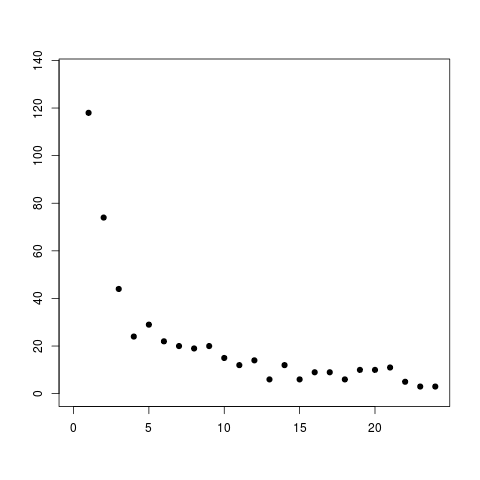
\epsfig{file = \figeco/FigFisher-0.ps, 
          height=.5\textwidth, width=0.6\textheight,  clip=, angle=270} \\
        \onslide<3>
        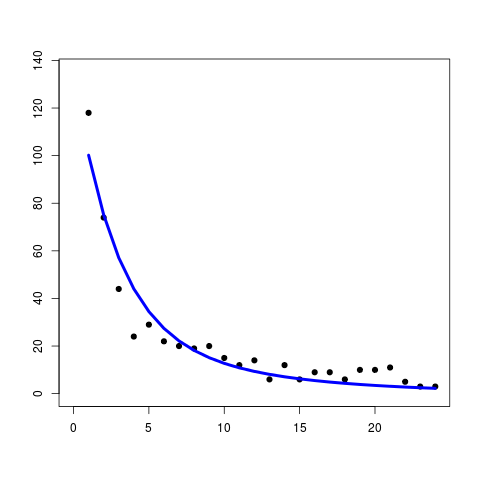
\epsfig{file = \figeco/FigFisher-1.ps, 
          height=.5\textwidth, width=0.6\textheight,  clip=, angle=270} \\
        \onslide<4->
        \epsfig{file = \figeco/FigFisher-2.ps, 
          height=.5\textwidth, width=0.6\textheight,  clip=, angle=270} \\
      \end{overprint}
    \end{tabular}
  \end{tabular}
  
  \onslide+<5->{
    \bigskip
    \paragraph{'Non parametric'=} parametric mixture
    $
    g(\cdot) = \sum_k \pi_k f_k(\cdot).
    $
  }
}

%--------------------------------------------------------------------
\frame{\frametitle{Model averaging}
  
  \begin{tabular}{cc}
    \hspace{-.5cm}
    \begin{tabular}{p{.45\textwidth}}
       \paragraph{Mixture.} For $K = 1... K_{\max}$ we get
       $\widehat{S}_K(0)$ and 
       $$
       Q_K(S(0)) \approx 
       P(S_K(0) |K, \Xbf)
       $$

       \bigskip
       \paragraph{Model averaging.} The estimates can be combined
       $$
       \widehat{S}(0) = \sum_K w_k \widehat{S}_K(0).
       $$
    \end{tabular}
    & 
    \hspace{-.5cm}
    \begin{tabular}{p{.5\textwidth}}
       \epsfig{file = \figeco/LDR12-Fig1.eps, 
         height=.5\textheight, width=0.5\textwidth,  clip=}
    \end{tabular}
  \end{tabular}
  
  \bigskip\pause
  \paragraph{Question:} Can we use variational Bayes E-M approximate posterior to get a credibility interval?
}

%--------------------------------------------------------------------
\frame{\frametitle{Importance sampling}

  \paragraph{Estimation an integral.} To define a confidence interval, we need to compute
  $$
  \begin{array}{rclcl}
    P(\Delta \in A | \Xbf) 
    \onslide+<2->{& = & \displaystyle{\int_A P(\Delta|\Xbf)} }
    \onslide+<4->{& = & \displaystyle{\int_A  \frac{P(\Delta|\Xbf)}{Q(\Delta)} Q(\Delta)} } \\
    \\
    \onslide+<3>{& = & \displaystyle{\frac1B \sum_b \Ibb\{\Delta^b \in A)} }
    \onslide+<5->{& = & \displaystyle{\frac1B \sum_b \Ibb\{\Delta^b \in A) \frac{P(\Delta^b|\Xbf)}{Q(\Delta^b)}} } \\
    \\
    \onslide+<3>{&  & \displaystyle{\{\Delta^b\} \text{i.i.d.} \sim P(\Delta|\Xbf)} }
    \onslide+<5->{&  & \displaystyle{\{\Delta^b\} \text{i.i.d.} \sim Q(\Delta)} }
  \end{array}
  $$
  
  \onslide+<6->{\bigskip
    \paragraph{Question:} Can we use take the variational Bayes $Q$ for this? }
  
  \onslide+<7->{\bigskip
    \paragraph{Exercise:} Show that $P(\Delta|\Xbf)$ achieves the smallest variance among all $Q$'s.}
}

%--------------------------------------------------------------------
\frame{\frametitle{Back to the example}

  \begin{tabular}{cc}
    \hspace{-.5cm}
    \begin{tabular}{p{.45\textwidth}}
      \paragraph{Idea.} Use $Q$ as a proposal: $S^b(0)$ i.i.d. $\sim Q_K$, \refer{LDR12}
      $$
      \widehat{P}(S(0)|K) \propto \frac1B \sum_b \frac{P(S^b(0),
        \Xbf|K)}{Q_K(S^b(0))}.
      $$
      
      \bigskip
      \paragraph{Variational Bayes posterior} does not explore the
      whole range of the true posterior.  
    \end{tabular}
    & 
    \hspace{-.5cm}
    \begin{tabular}{p{.5\textwidth}}
      \epsfig{file = \figeco/LDR12-Fig2.eps, 
        height=.5\textheight, width=0.5\textwidth,  clip=} \\
    \end{tabular}
  \end{tabular}

  \bigskip\pause
%  \hspace{-0.5cm}
  \begin{tabular}{rrl}
    \paragraph{Variance inflation.} & Prior: & $\displaystyle{\Beta(a,
      b)}$ \\
    & Variational posterior: & $\displaystyle{\Beta(\widetilde{a},
      \widetilde{b})}$ \\
    & Inflated variational posterior: &
    $\displaystyle{\Beta\left({\widetilde{a}}/\emphase{v},
        {\widetilde{b}}/\emphase{v} \right)}$
  \end{tabular}
  }

%-------------------------------------------------------------------- 
\frame{\frametitle{Human gut microbiome}

  \begin{tabular}{cc}
    \hspace{-.5cm}
    \begin{tabular}{p{.5\textwidth}}
       3,180 recognized OTU \\
       ~\\
       \epsfig{file = \figeco/LDR10-42.eps, 
         height=.5\textheight, width=0.75\textwidth,  clip=} \\
       \\
      VBMA weights of geometric mixtures: 
      $w_4 = .971$, $w_3 = .026$.
    \end{tabular}
    & 
    \hspace{-.5cm}
    \begin{tabular}{p{.5\textwidth}}
      \pause
      Estimated $\#$ species: 25,700. \\
      ~\\
      \epsfig{file = \figeco/LDR12-Fig6.eps, 
        height=.5\textheight, width=0.45\textwidth,  clip=} \\
      \\
      $\text{CI}_{95\%} = [19,421; 36,355]$. \\
      ~
    \end{tabular}
  \end{tabular}
}

%--------------------------------------------------------------------
\section{Some conclusions}
%--------------------------------------------------------------------
\frame{\frametitle{Some conclusions}

  \paragraph{Variational approximation.}
  \begin{itemize}
  \item Reasonably easy tool to get approximate conditional distributions;
  \item More scalable than standard MCMC (?);
  \item Few general theoretical guaranties;
  \item Happens to be efficient in some specific frameworks (e.g. graphs, due a specific asymtotic framework\footnote{not true for sparse graphs});
  \item Can be combined with MCMC approaches.
  \end{itemize}

  }

%--------------------------------------------------------------------
{\tiny
  \bibliography{/home/robin/Biblio/ARC,/home/robin/Biblio/AST}
  % ,/Biblio/SSB} 
  \bibliographystyle{/home/robin/LATEX/astats}
  %\bibliographystyle{plain}
  }

%--------------------------------------------------------------------
\appendix
%-------------------------------------------------------------------- 
\section{Appendix}

%--------------------------------------------------------------------
%--------------------------------------------------------------------
\end{document}
%--------------------------------------------------------------------
%--------------------------------------------------------------------

  \begin{tabular}{cc}
    \hspace{-.5cm}
    \begin{tabular}{p{.5\textwidth}}
    \end{tabular}
    & 
    \hspace{-.5cm}
    \begin{tabular}{p{.5\textwidth}}
    \end{tabular}
  \end{tabular}
